\chapter{Pengujian}

\begin{figure}[ht]
  \centering
  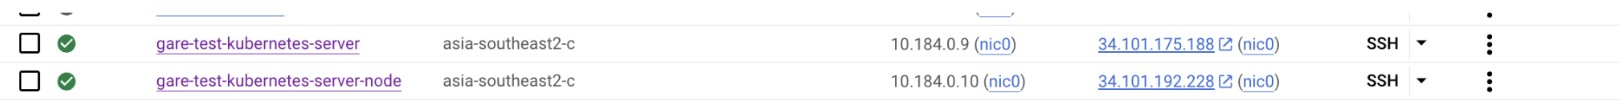
\includegraphics[width=0.8\textwidth]{resources/chapter-4/pengujian/kube-gcp-01.jpg}
  \caption{Hasil Pembuatan Virtual Machine pada GCP}
  \label{fig:hasil-pembuatan-virtual-machine-gcp}
\end{figure}

\begin{figure}[ht]
  \centering
  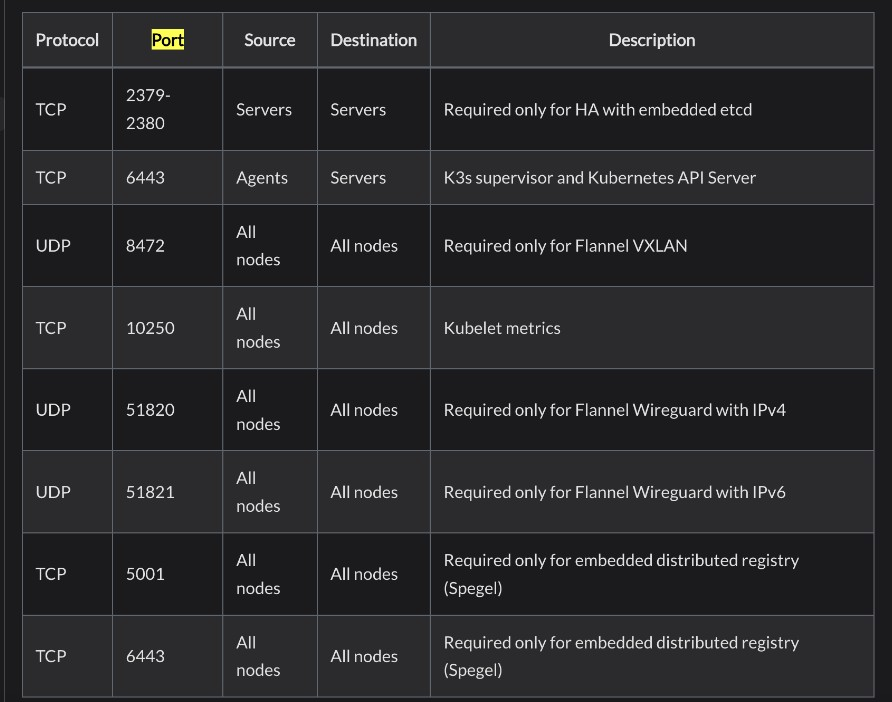
\includegraphics[width=0.8\textwidth]{resources/chapter-4/pengujian/kube-gcp-03.jpg}
  \caption{Daftar Kegunaan Port}
  \label{fig:daftar-kegunaan-port}
\end{figure}

\begin{figure}[ht]
  \centering
  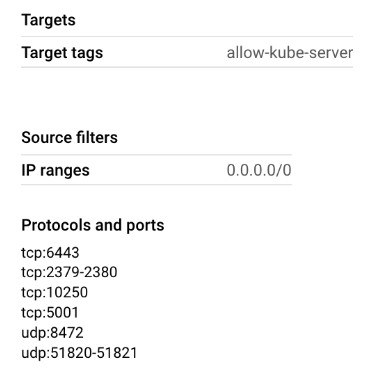
\includegraphics[width=0.8\textwidth]{resources/chapter-4/pengujian/kube-gcp-02.jpg}
  \caption{Hasil Firewall Rule pada GCP}
  \label{fig:hasil-firewall-rule-pada-gcp}
\end{figure}

\begin{figure}[ht]
  \centering
  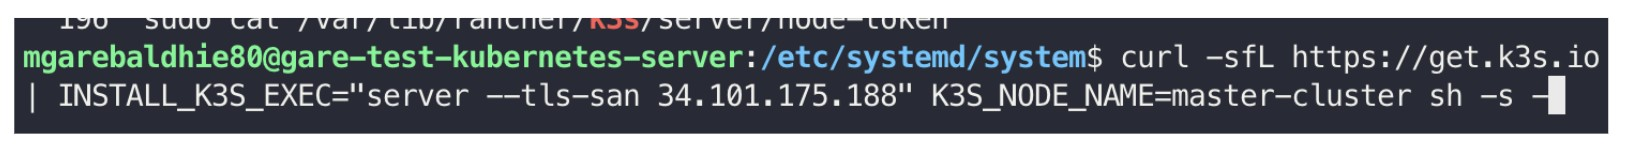
\includegraphics[width=0.8\textwidth]{resources/chapter-4/pengujian/kube-gcp-04.jpg}
  \caption{Instalasi Master Node di \textit{Virtual Machine}}
  \label{fig:instalasi-master-node-gcp}
\end{figure}

\begin{figure}[ht]
  \centering
  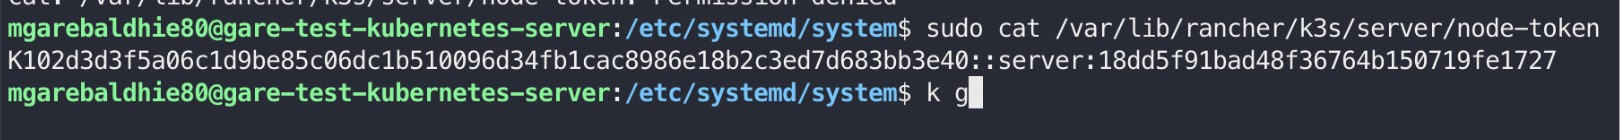
\includegraphics[width=0.8\textwidth]{resources/chapter-4/pengujian/kube-gcp-05.jpg}
  \caption{Pengambilan Token Registrasi Cluster}
  \label{fig:pengambilan-token-registrasi-cluster}
\end{figure}

\begin{figure}[ht]
  \centering
  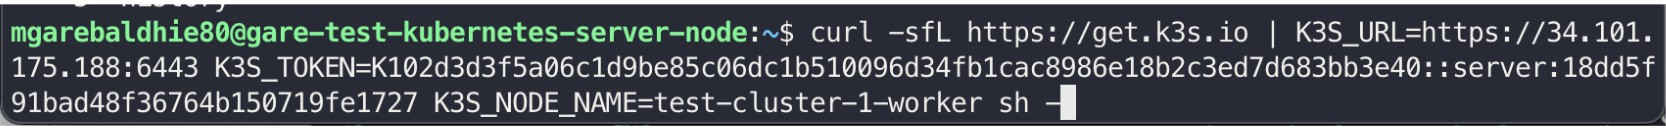
\includegraphics[width=0.8\textwidth]{resources/chapter-4/pengujian/kube-gcp-06.jpg}
  \caption{Instalasi Worker Node di \textit{Virtual Machine}}
  \label{fig:instalasi-worker-node-gcp}
\end{figure}

\begin{figure}[ht]
  \centering
  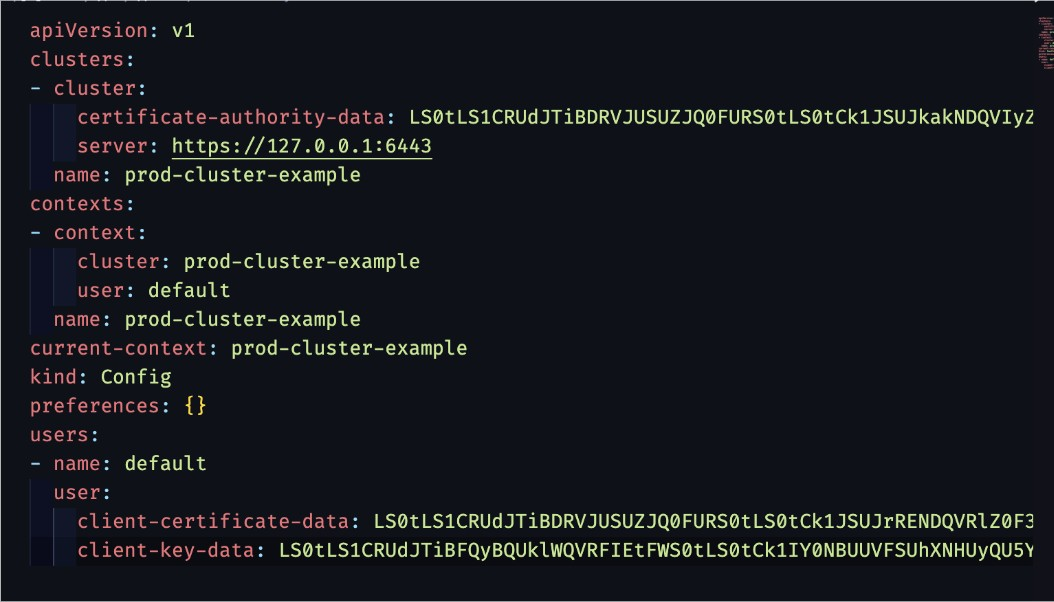
\includegraphics[width=0.8\textwidth]{resources/chapter-4/pengujian/kube-gcp-07.jpg}
  \caption{Konfigurasi \textit{Cluster} pada \textit{Master Node GCP}}
  \label{fig:konfigurasi-cluster-master-node-gcp}
\end{figure}

\begin{figure}[ht]
  \centering
  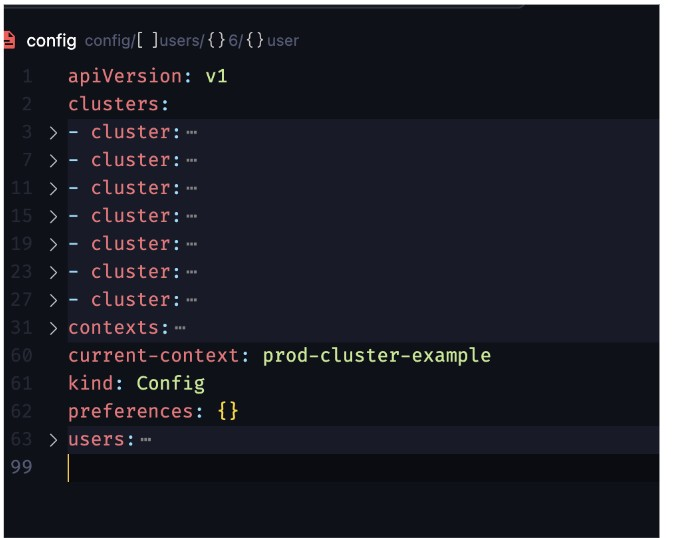
\includegraphics[width=0.8\textwidth]{resources/chapter-4/pengujian/kube-gcp-08.jpg}
  \caption{Pemindahan Konfigurasi \textit{Cluster} pada \textit{Master Node GCP}}
  \label{fig:proses-pemindahan-konfigurasi-master-gcp}
\end{figure}

\begin{figure}[ht]
  \centering
  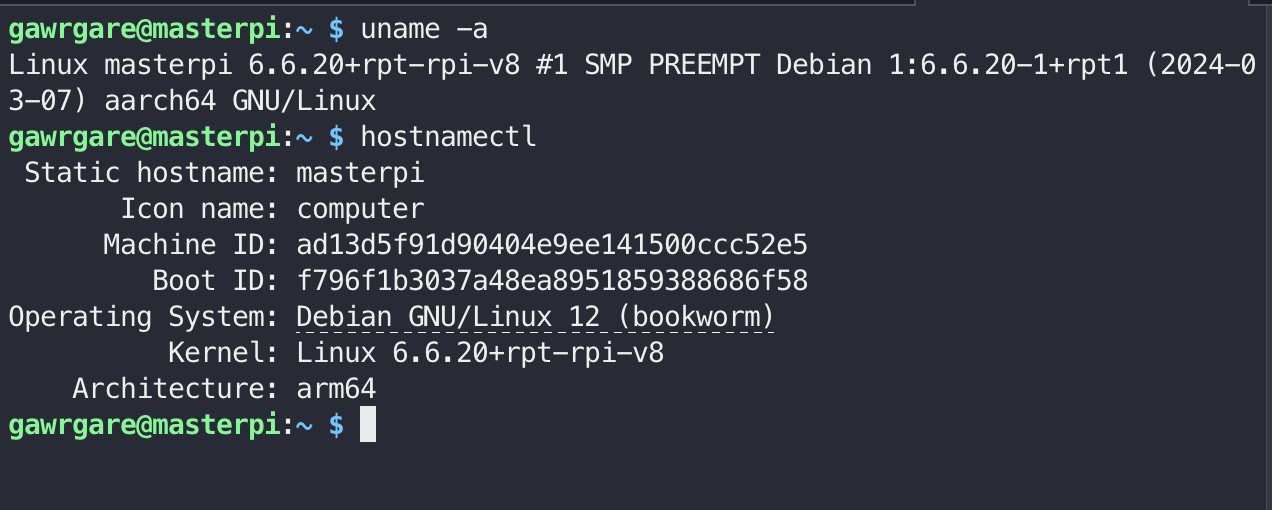
\includegraphics[width=0.8\textwidth]{resources/chapter-4/pengujian/raspi-01.jpg}
  \caption{Hostname Raspsi Master Nodes}
  \label{fig:hostname-raspi-master-nodes}
\end{figure}

\begin{figure}[ht]
  \centering
  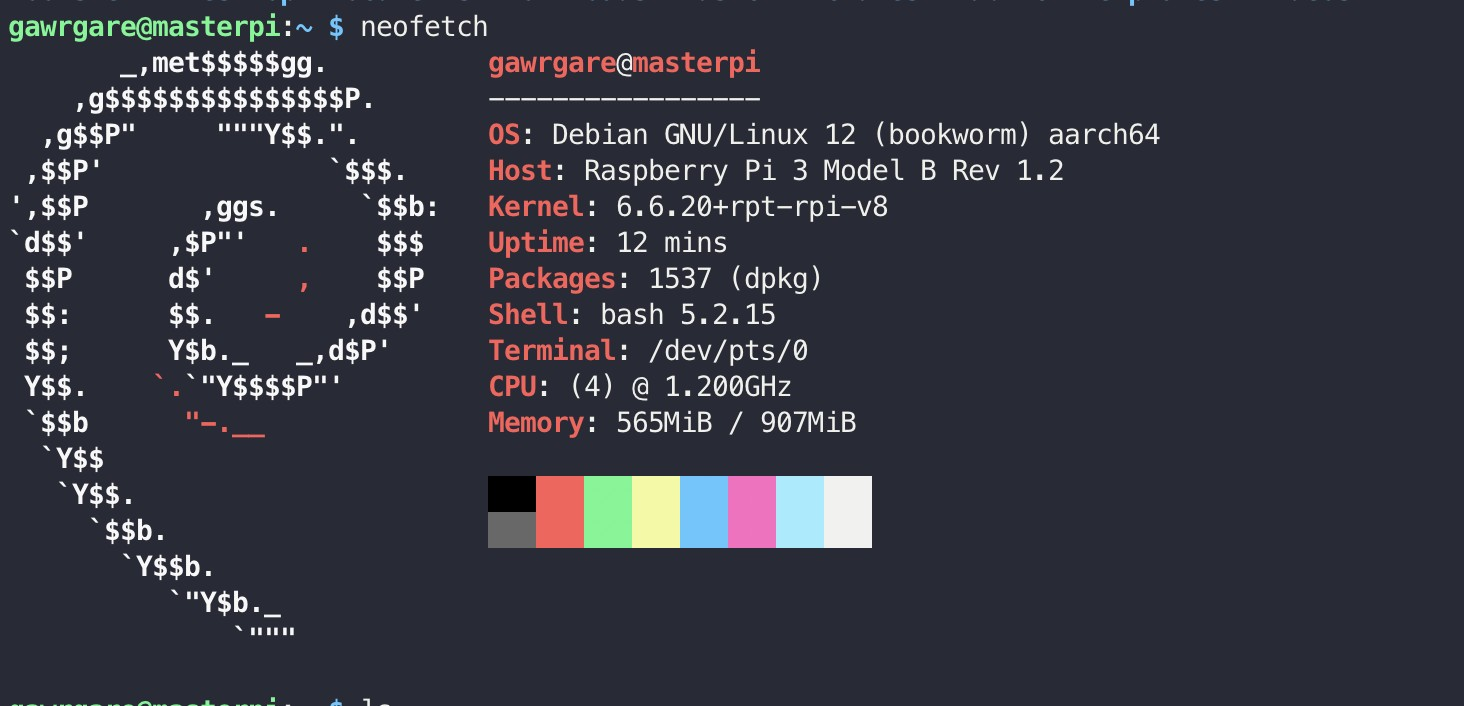
\includegraphics[width=0.8\textwidth]{resources/chapter-4/pengujian/raspi-master-neofetch.jpg}
  \caption{Spesifikasi Raspsi Master Nodes}
  \label{fig:spesifikasi-raspi-master-nodes}
\end{figure}

\begin{figure}[ht]
  \centering
  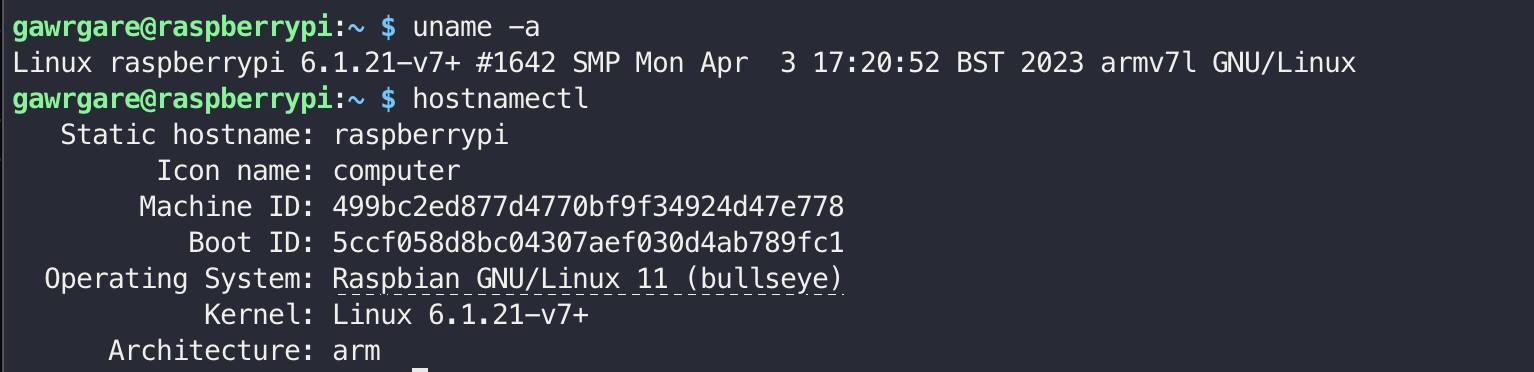
\includegraphics[width=0.8\textwidth]{resources/chapter-4/pengujian/raspi-01-worker.jpg}
  \caption{Hostname Raspsi Worker Nodes}
  \label{fig:hostname-raspi-worker-nodes}
\end{figure}

\begin{figure}[ht]
  \centering
  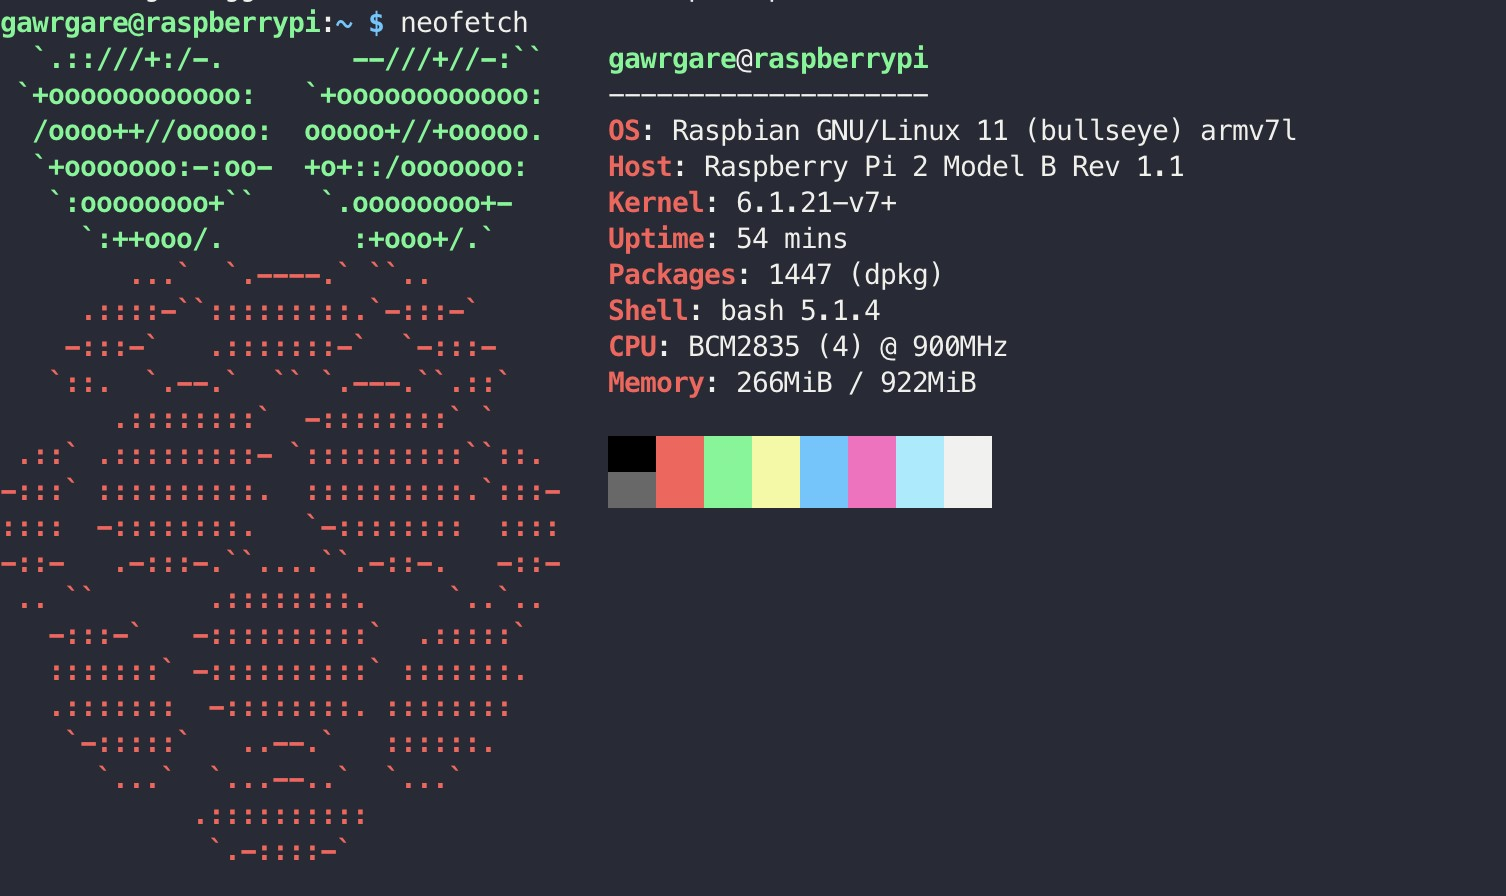
\includegraphics[width=0.8\textwidth]{resources/chapter-4/pengujian/raspi-worker-neofetch.jpg}
  \caption{Spesifikasi Raspsi Worker Nodes}
  \label{fig:spesifikasi-raspi-worker-nodes}
\end{figure}

\begin{figure}[ht]
  \centering
  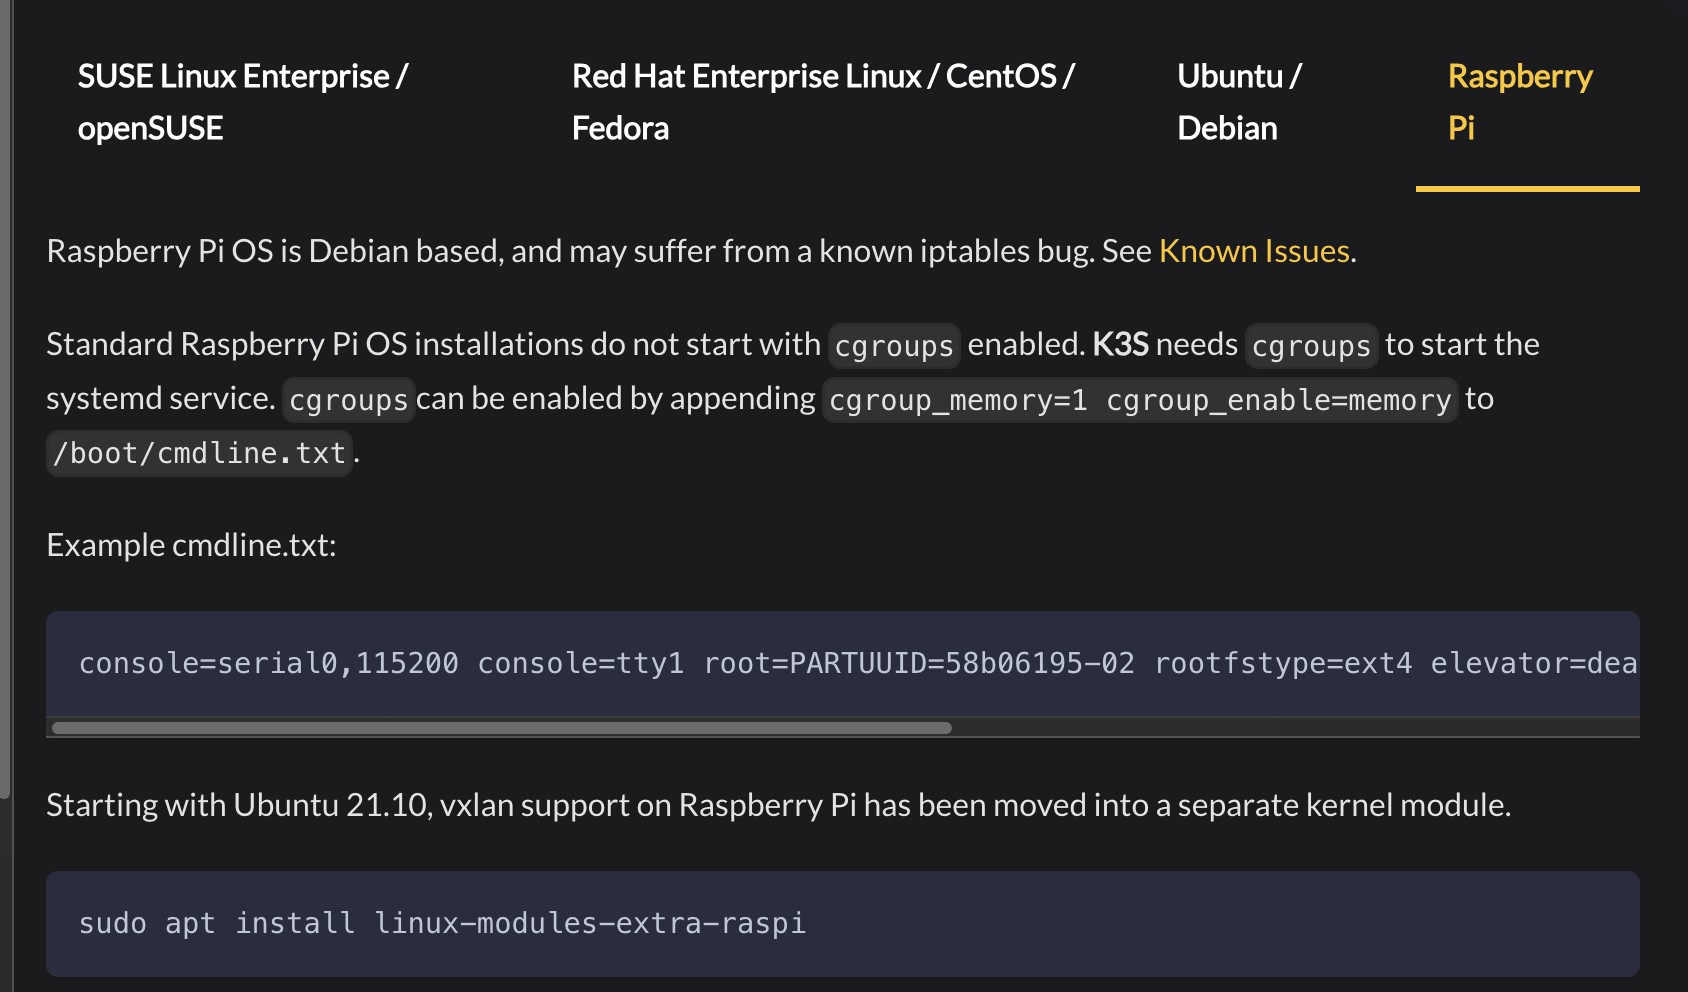
\includegraphics[width=0.8\textwidth]{resources/chapter-4/pengujian/raspi-02-additional.jpg}
  \caption{\textit{Additional Command} untuk RaspberryPi}
  \label{fig:additional-command-raspberrypi}
\end{figure}

\begin{figure}[ht]
  \centering
  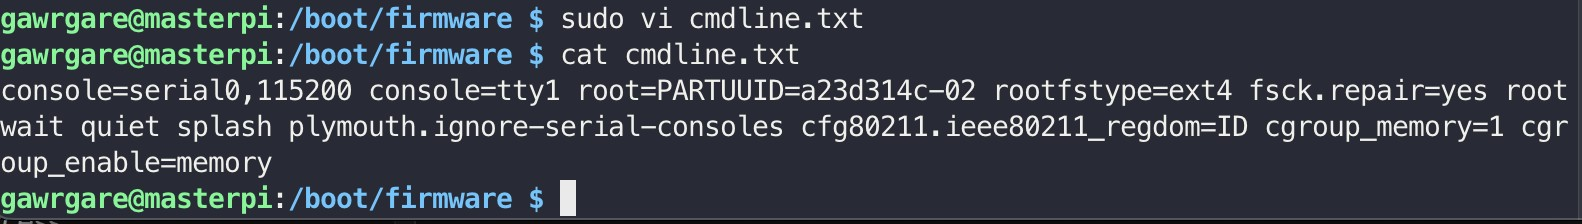
\includegraphics[width=0.8\textwidth]{resources/chapter-4/pengujian/raspi-02-additional-02.jpg}
  \caption{Penambahan \textit{cgroups} pada \textit{Cmdline}}
  \label{fig:penambahan-cgroups-pada-cmdline}
\end{figure}

\begin{figure}[ht]
  \centering
  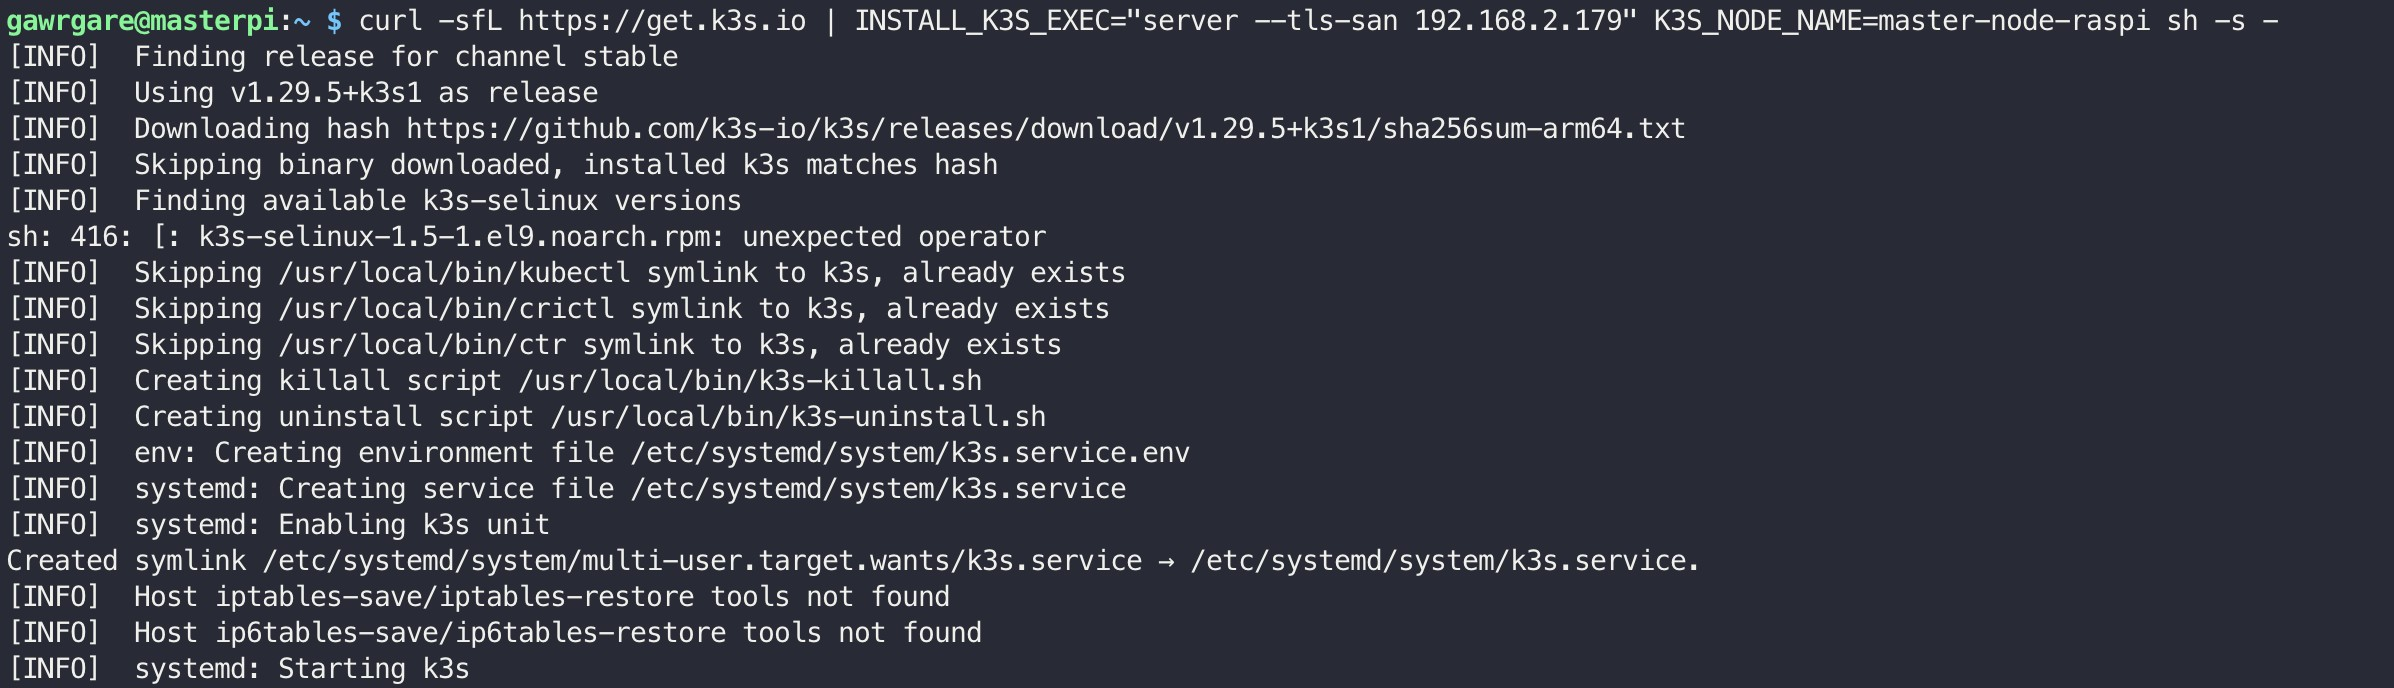
\includegraphics[width=0.8\textwidth]{resources/chapter-4/pengujian/raspi-03.jpg}
  \caption{Instalasi Master Raspi \textit{Node}}
  \label{fig:instalasi-master-raspi-nodes}
\end{figure}

\begin{figure}[ht]
  \centering
  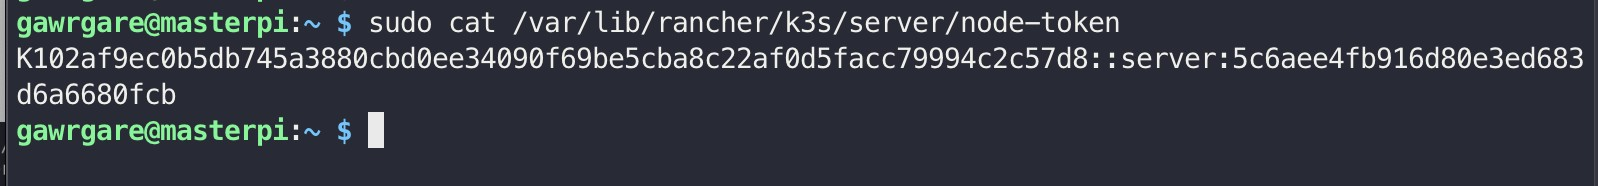
\includegraphics[width=0.8\textwidth]{resources/chapter-4/pengujian/raspi-token-gen.jpg}
  \caption{Master Raspi Generate Token}
  \label{fig:raspi-master-gen-token}
\end{figure}

\begin{figure}[ht]
  \centering
  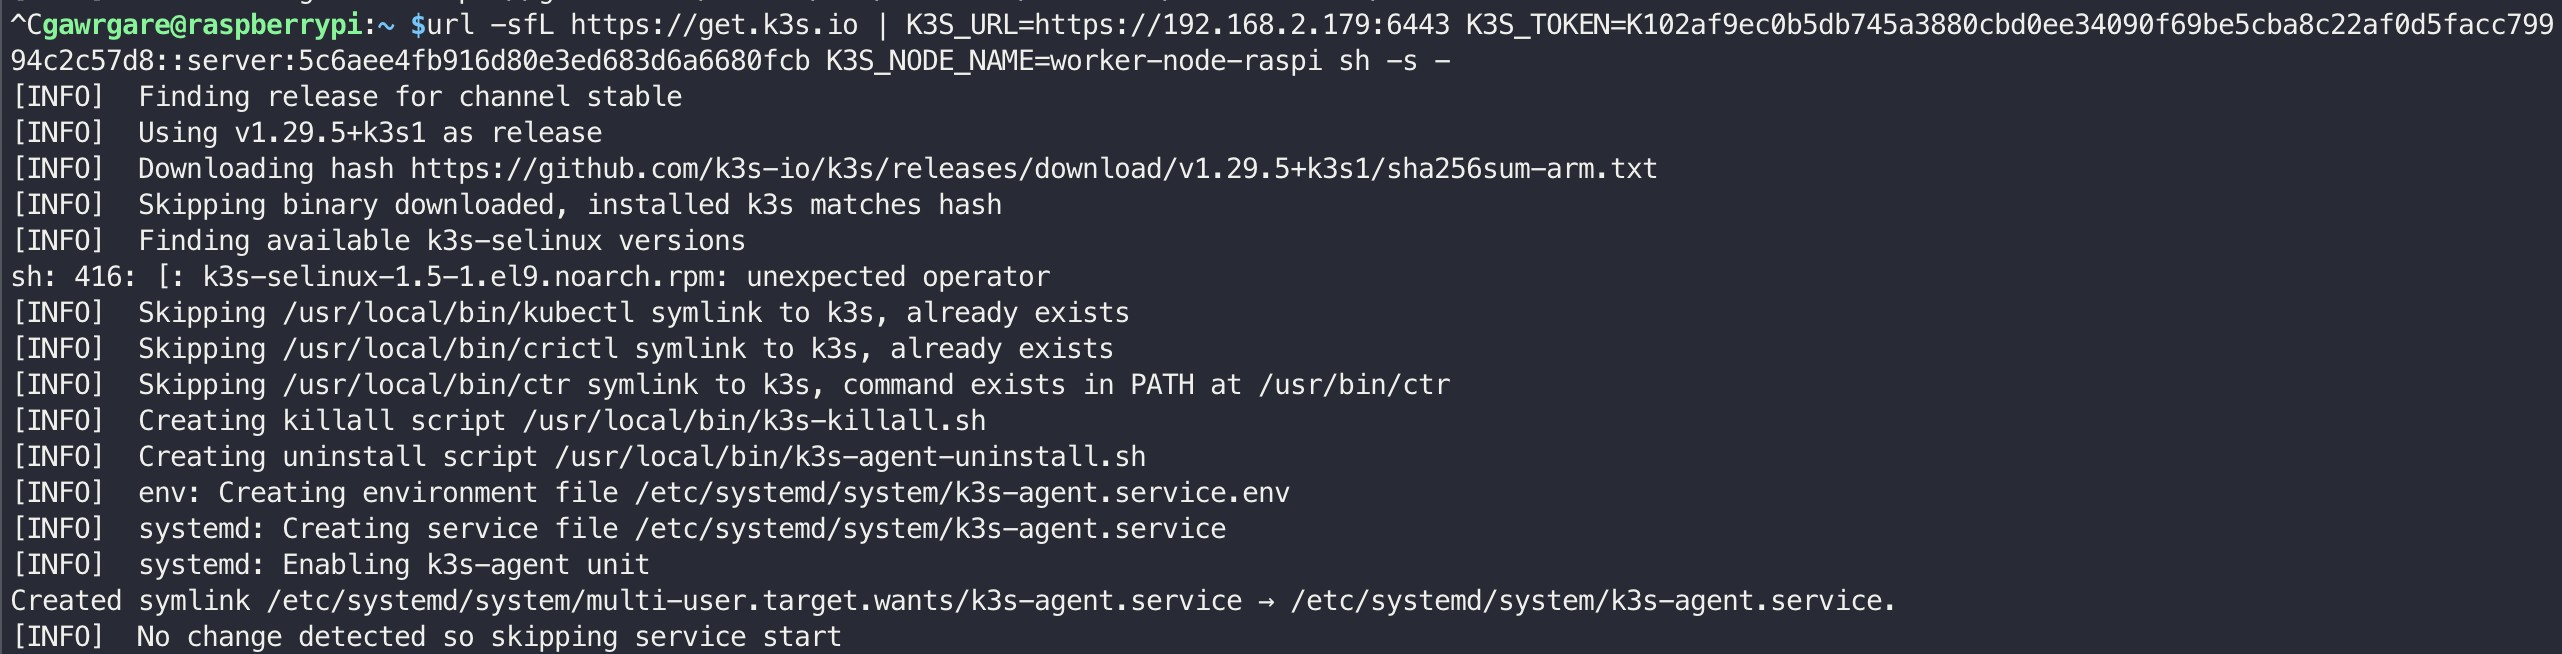
\includegraphics[width=0.8\textwidth]{resources/chapter-4/pengujian/raspi-04.jpg}
  \caption{Instalasi Worker Raspi \textit{Node}}
  \label{fig:instalasi-worker-raspi-node}
\end{figure}

\begin{figure}[ht]
  \centering
  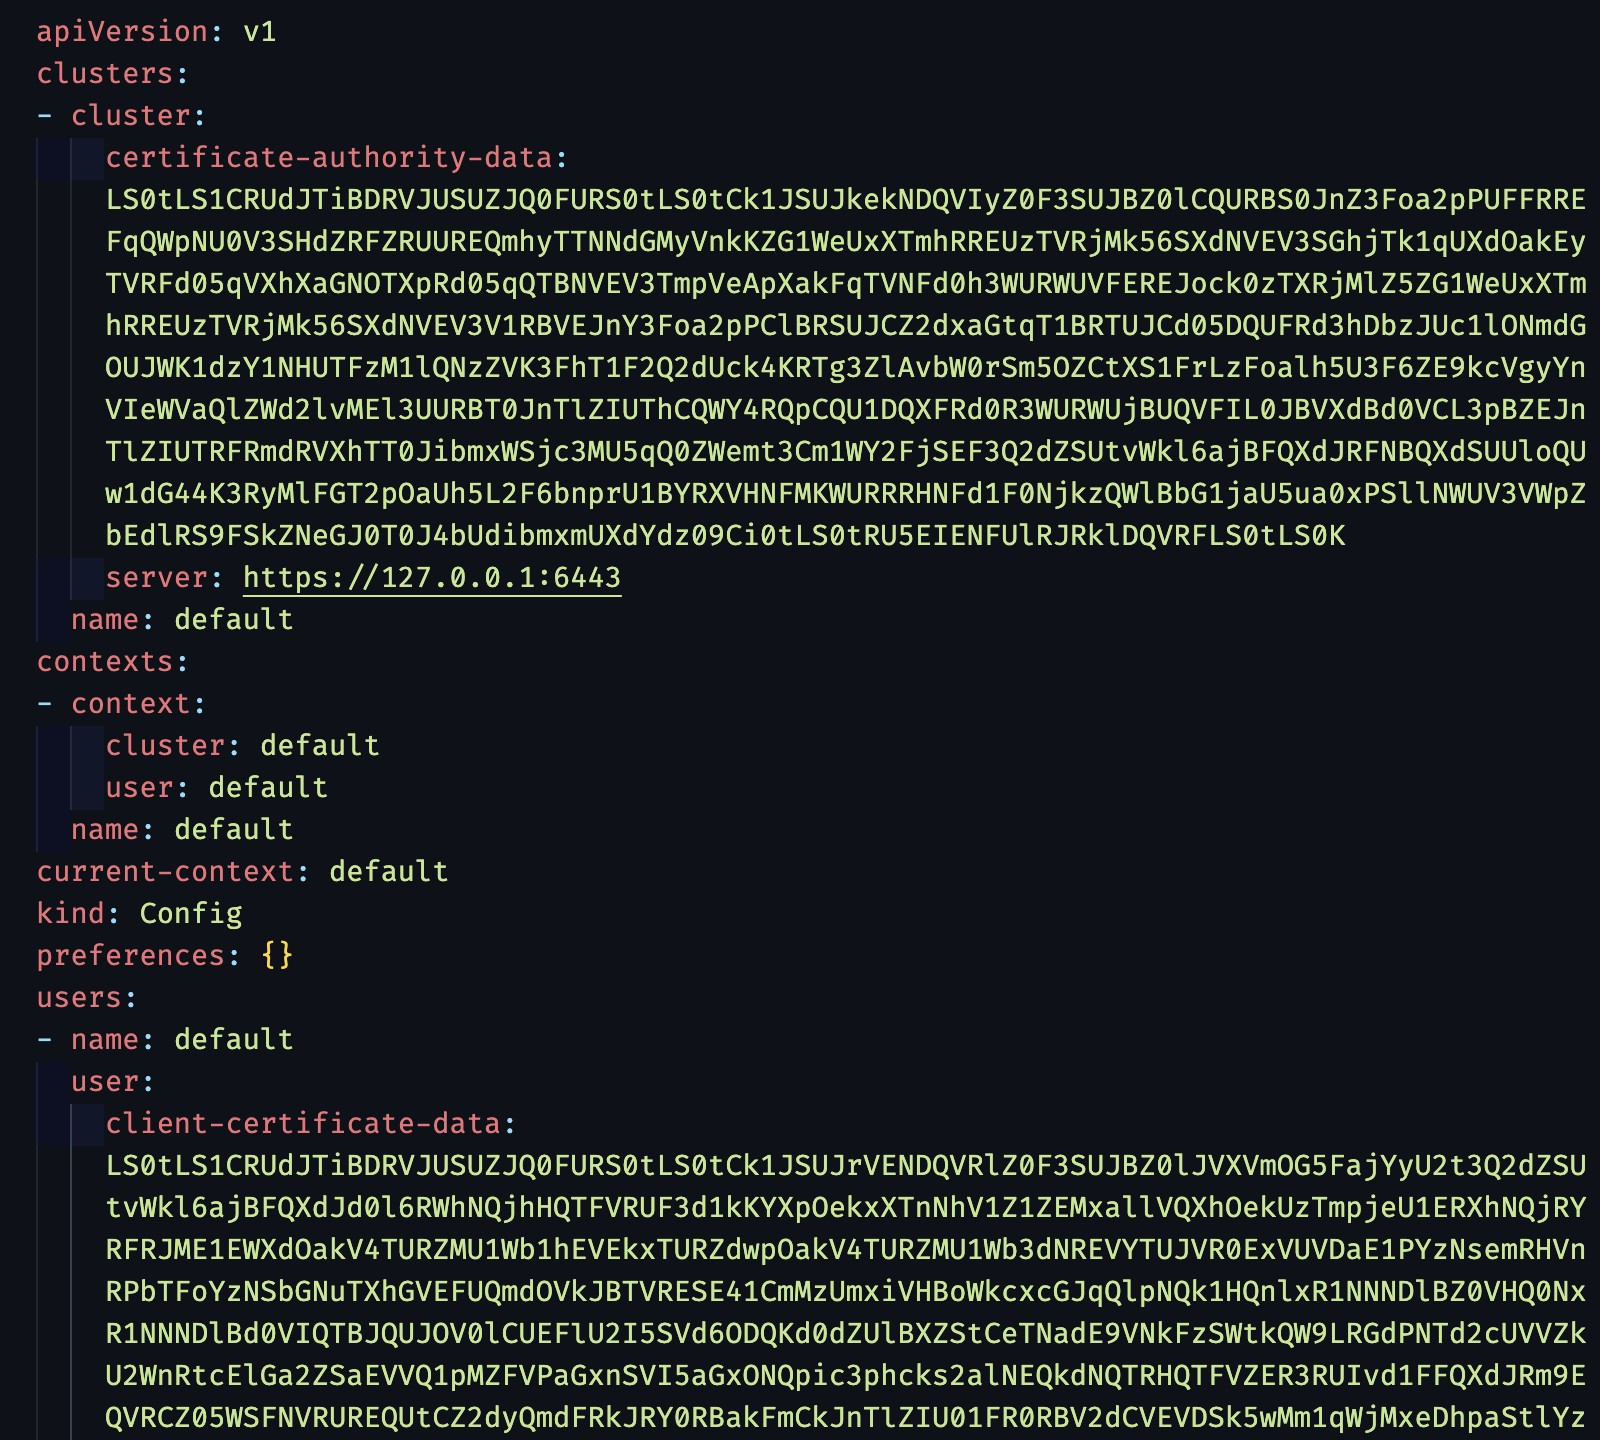
\includegraphics[width=0.8\textwidth]{resources/chapter-4/pengujian/raspi-kube-config.jpg}
  \caption{Kubernetes Config RaspberryPi}
  \label{fig:raspi-kube-config}
\end{figure}

\begin{figure}[ht]
  \centering
  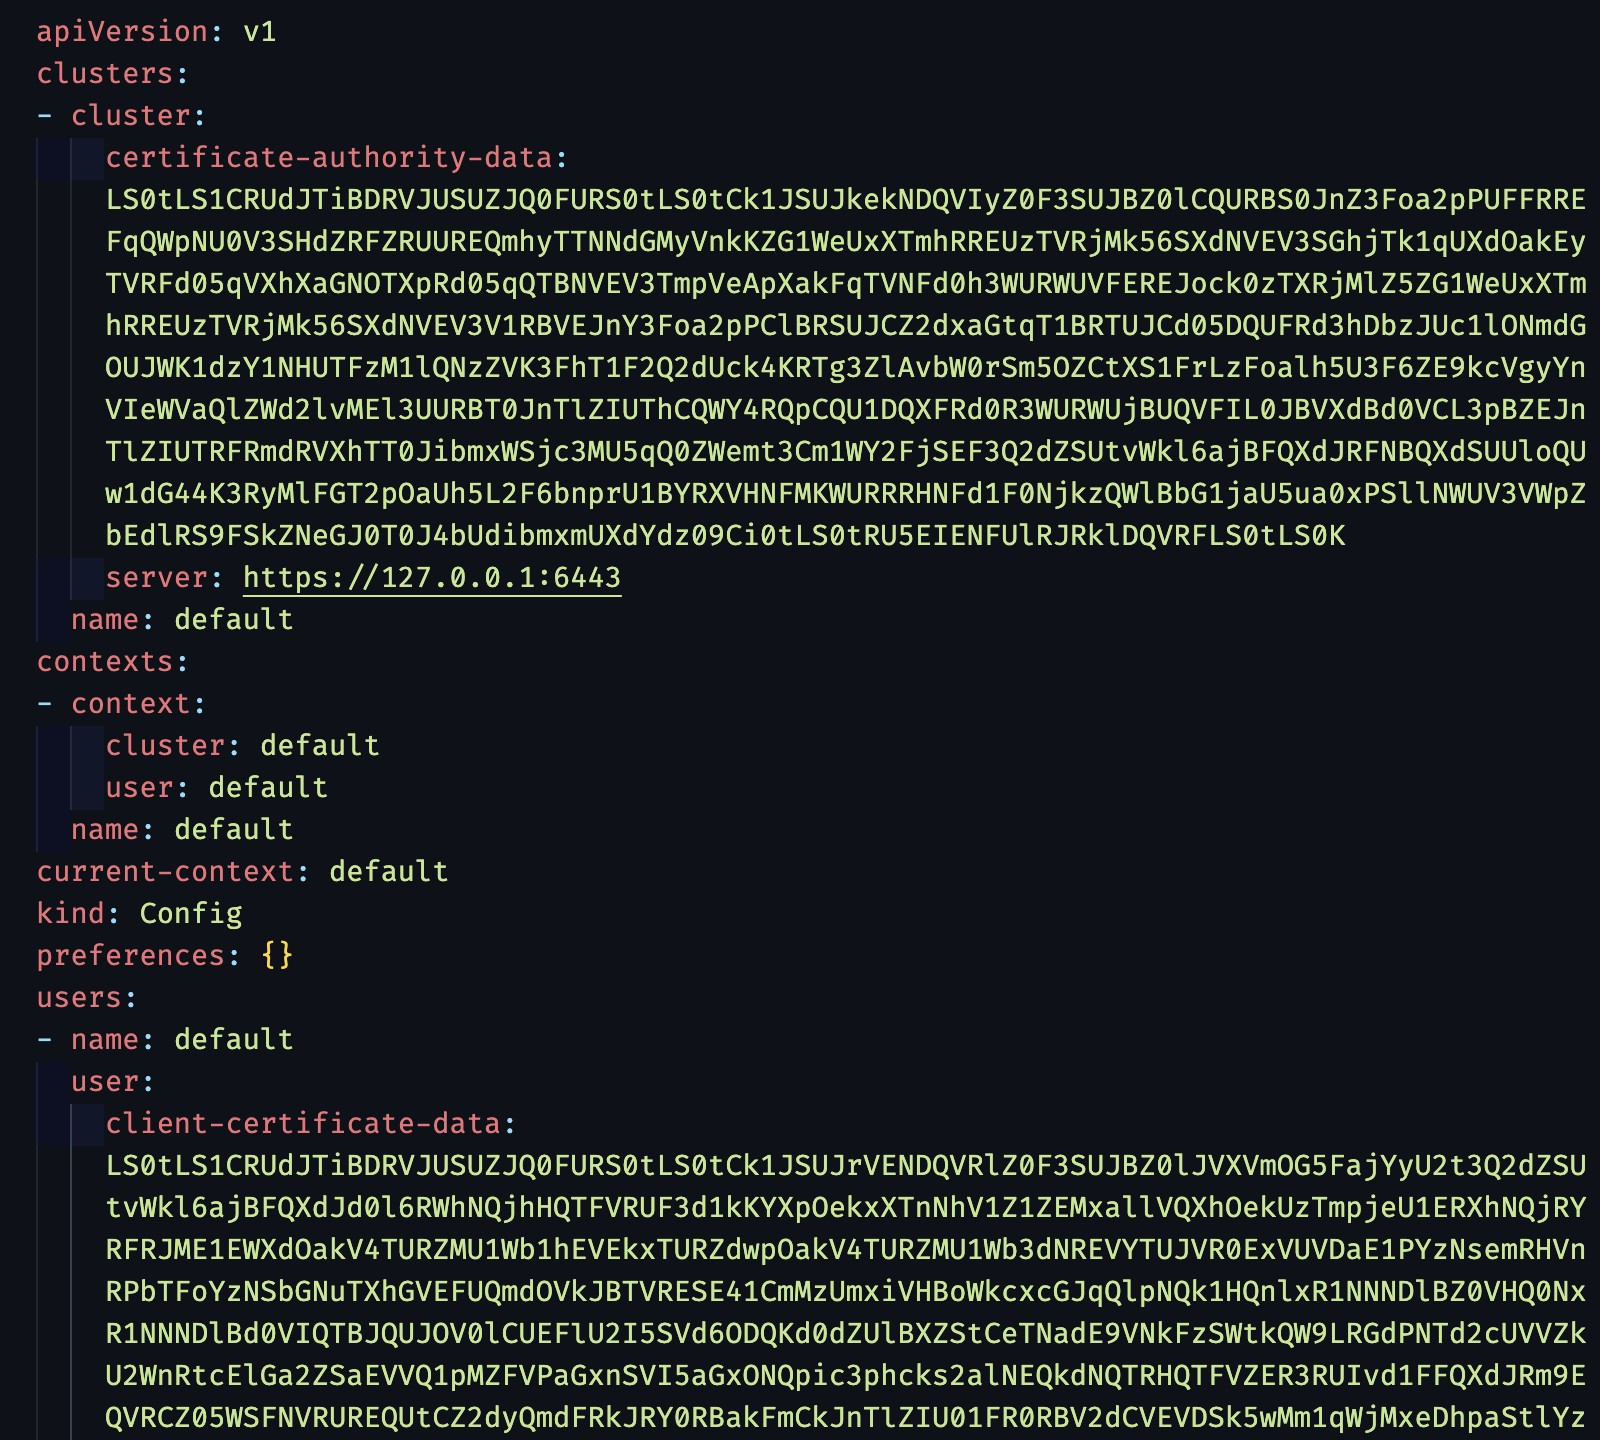
\includegraphics[width=0.8\textwidth]{resources/chapter-4/pengujian/raspi-kube-config.jpg}
  \caption{Menambagkan Kubernetes Config RaspberryPi pada Sistem}
  \label{fig:raspi-add-kubeconfig}
\end{figure}

\begin{figure}[ht]
  \centering
  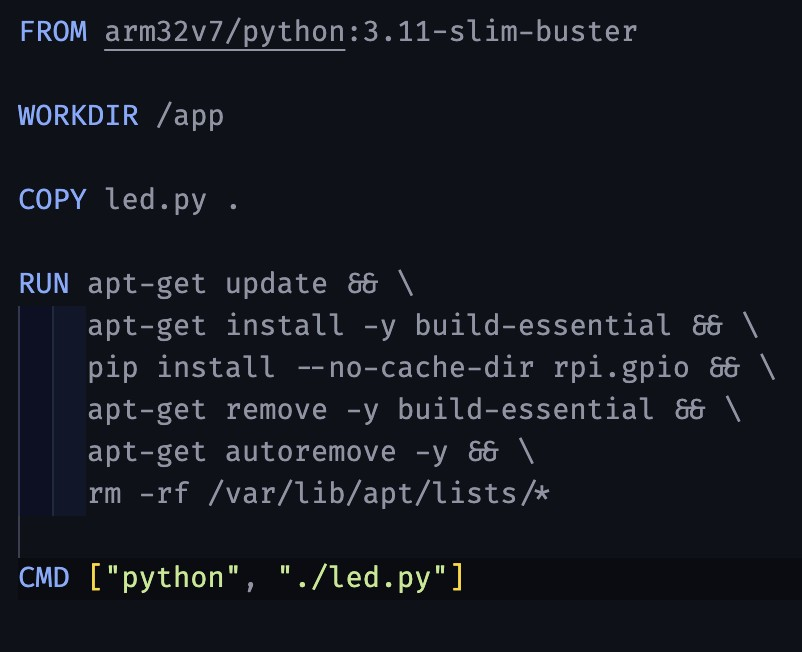
\includegraphics[width=0.8\textwidth]{resources/chapter-4/pengujian/pengujian-sistem-raspi-09-dockerfile.jpg}
  \caption{Python Docker LED Script}
  \label{fig:raspi-docker-led-script}
\end{figure}

\begin{figure}[ht]
  \centering
  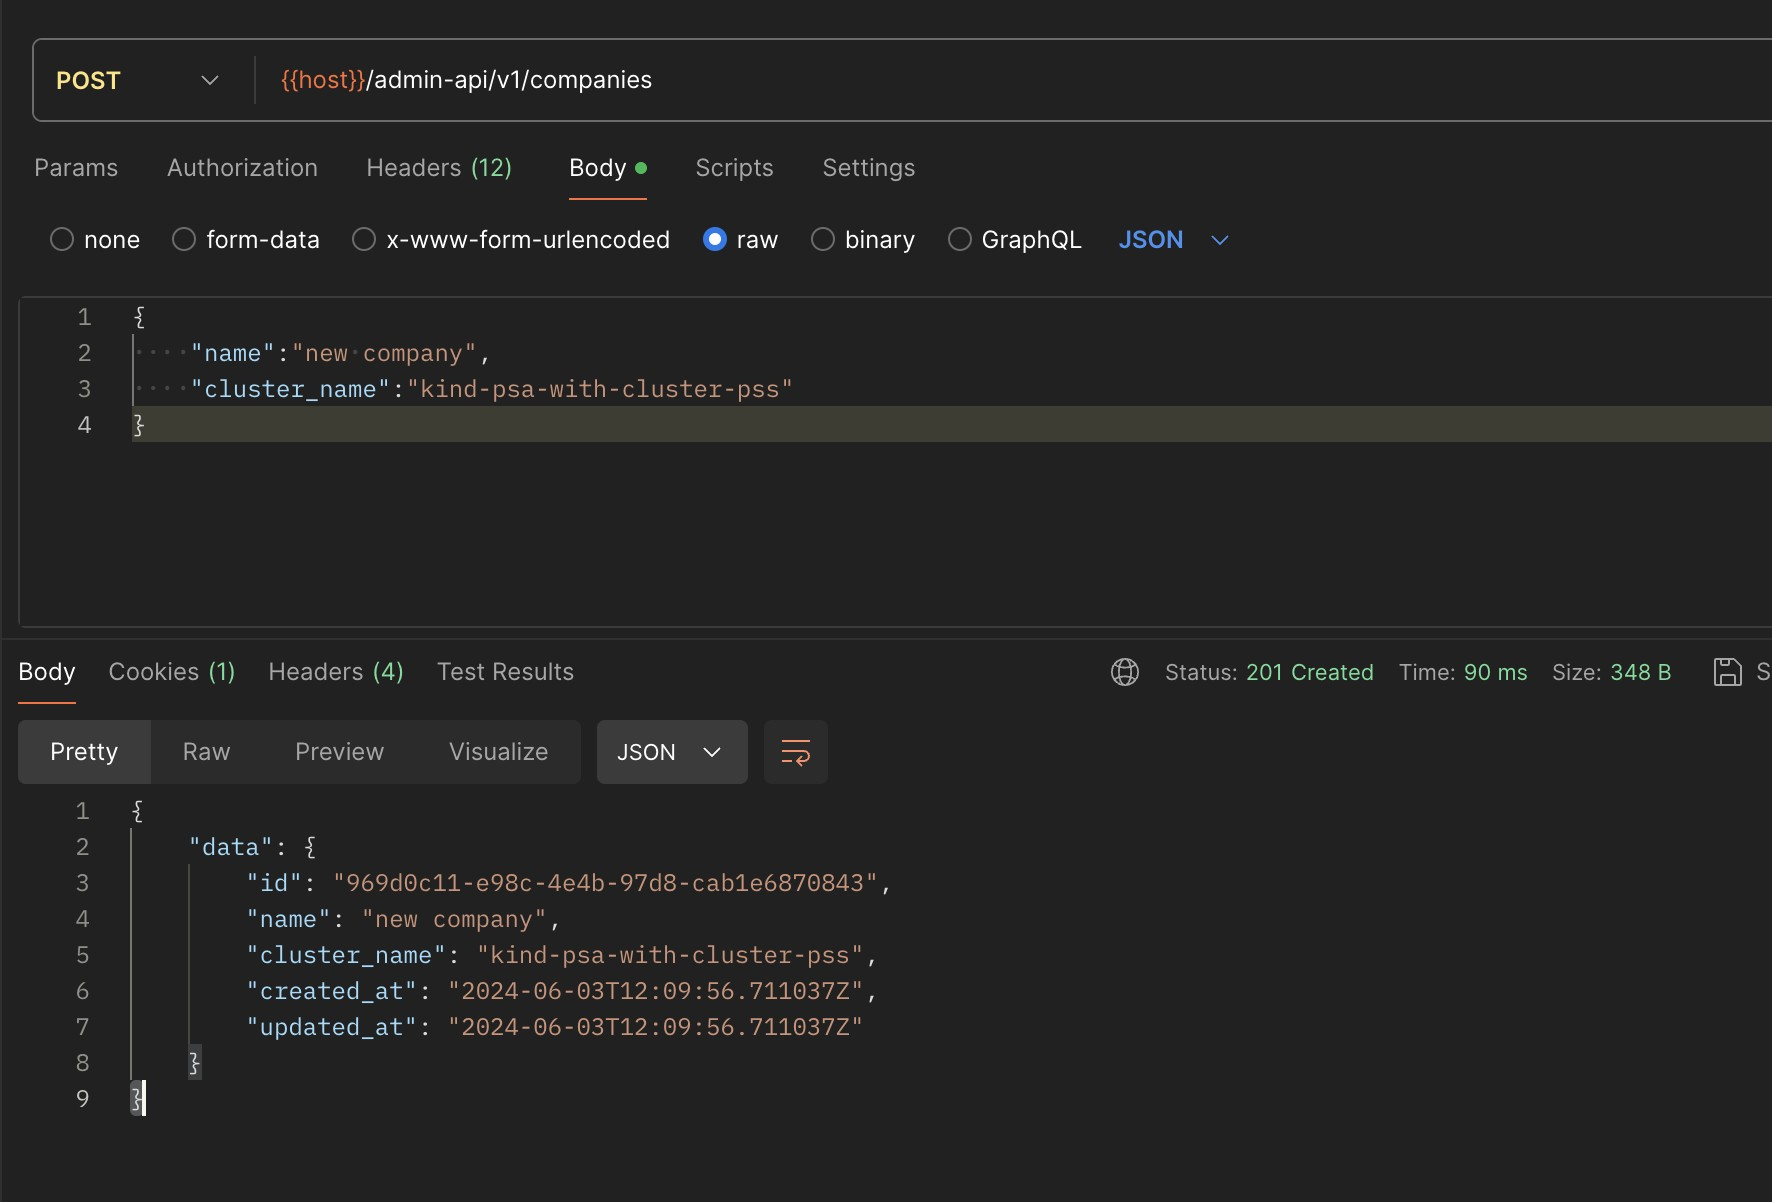
\includegraphics[width=0.8\textwidth]{resources/chapter-4/pengujian/p01.jpg}
  \caption{\textit{Request dan Response Pengujian} P01}
  \label{fig:pengujian-p01}
\end{figure}

\begin{figure}[ht]
  \centering
  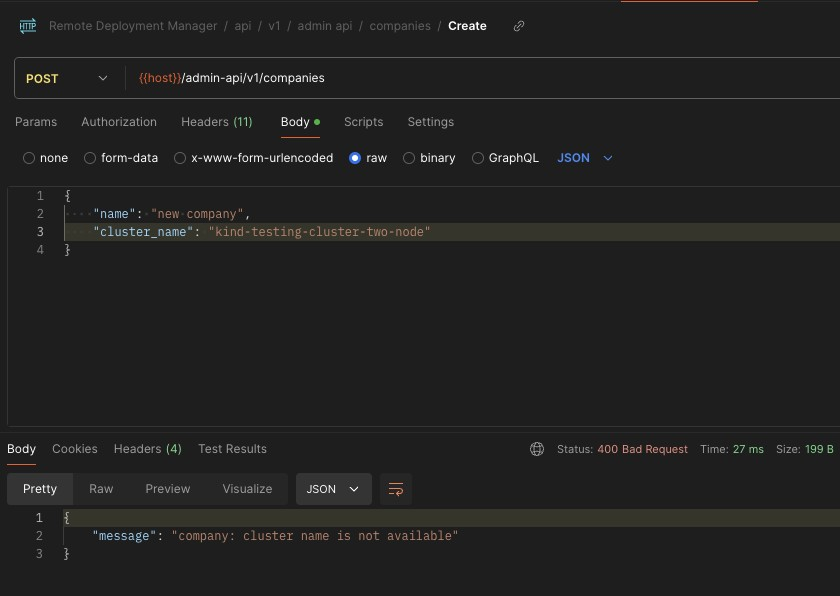
\includegraphics[width=0.8\textwidth]{resources/chapter-4/pengujian/p02.jpg}
  \caption{\textit{Request dan Response Pengujian} P02}
  \label{fig:pengujian-p02}
\end{figure}

\begin{figure}[ht]
  \centering
  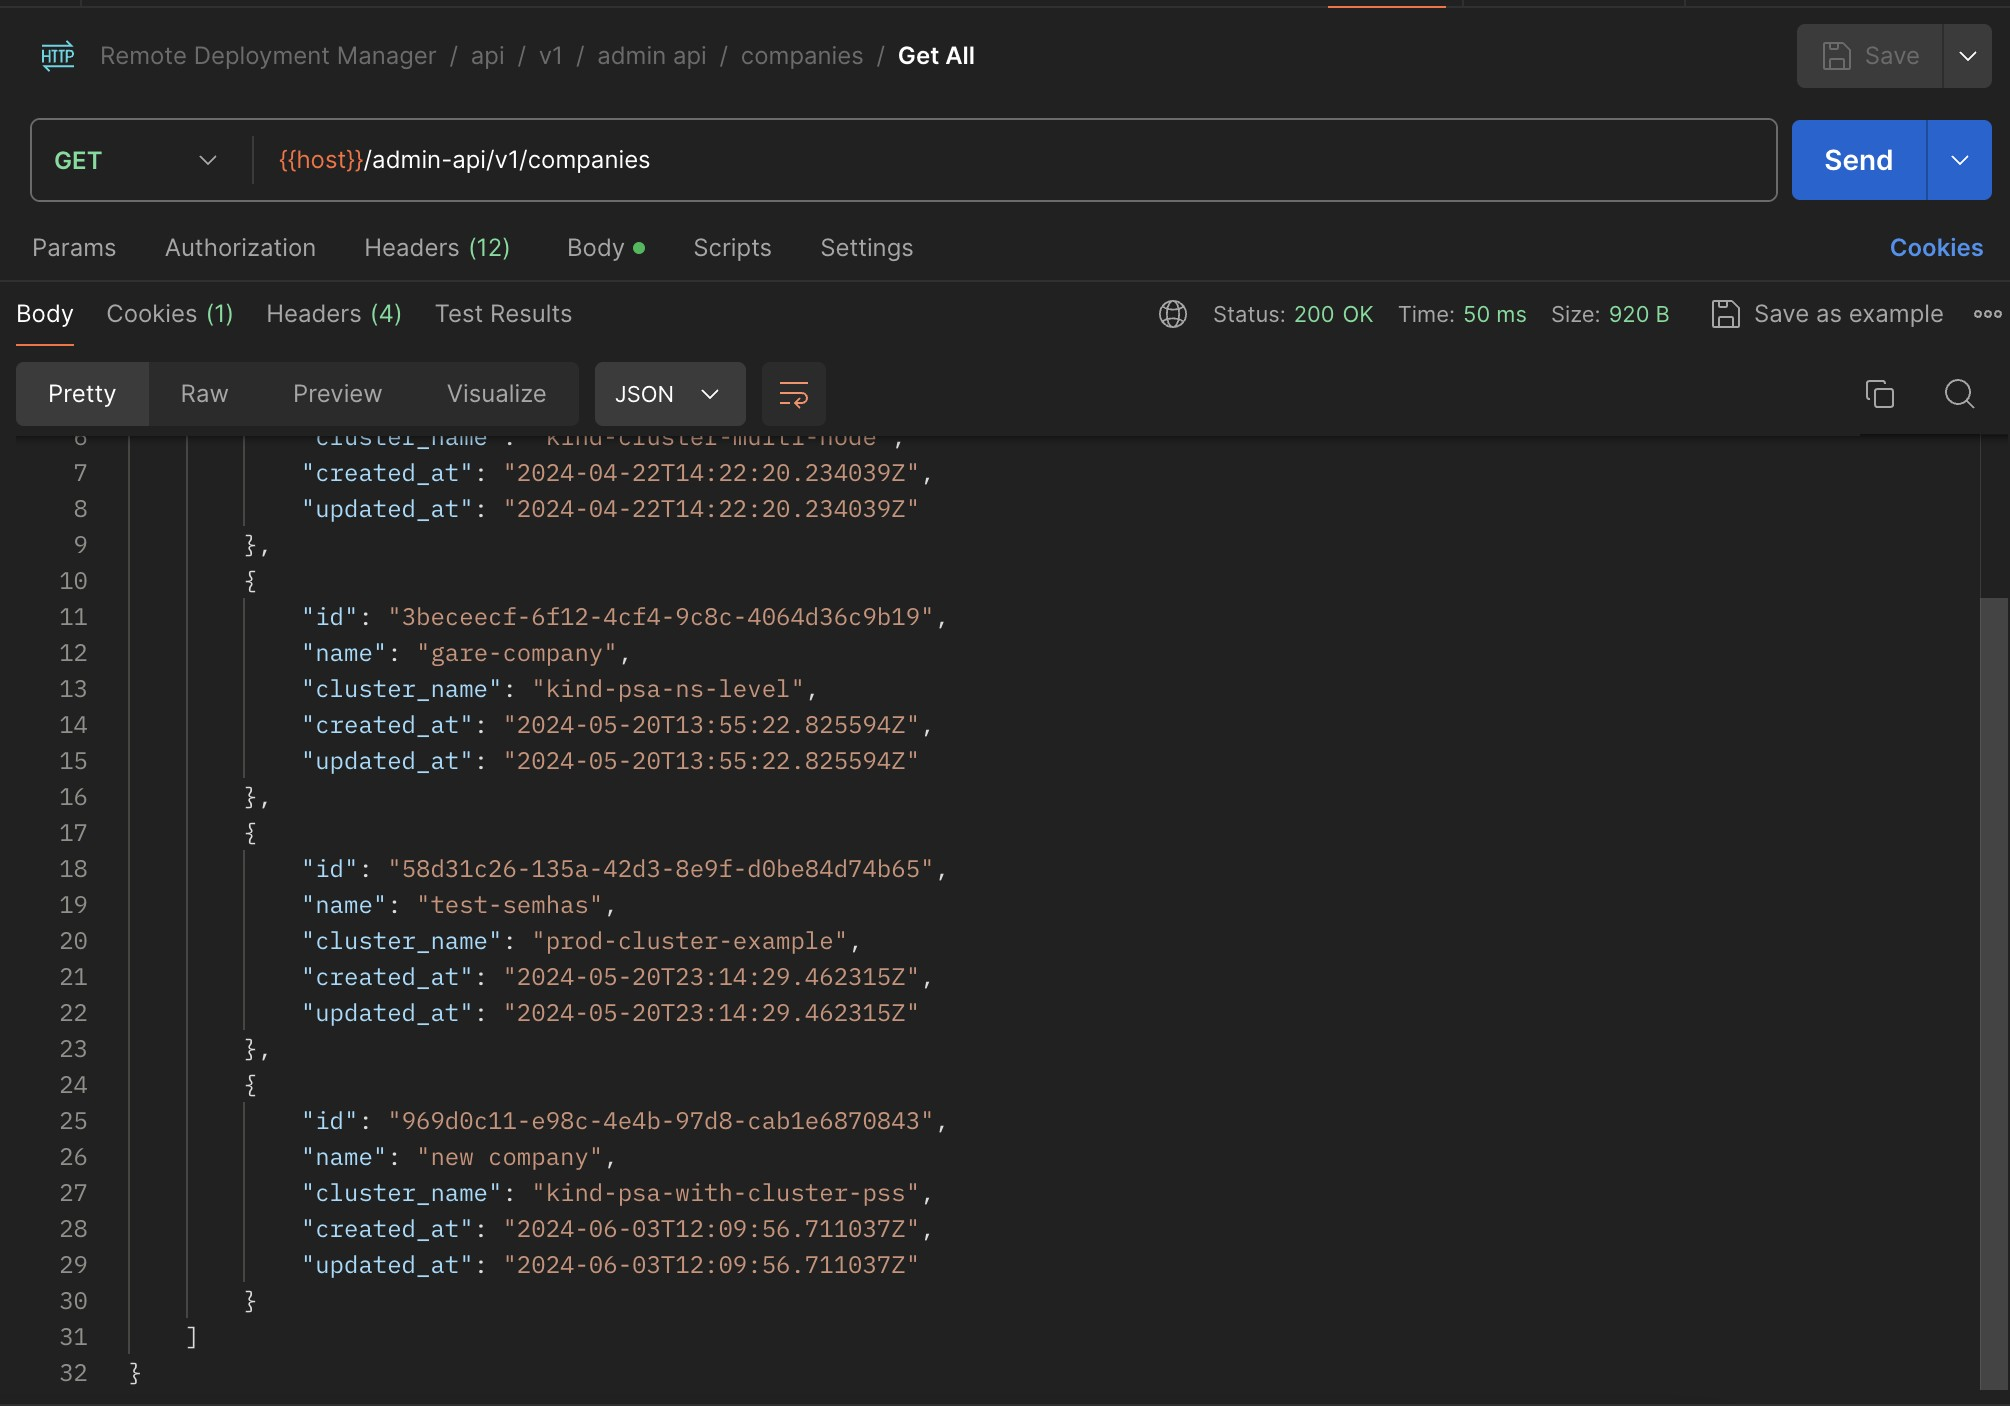
\includegraphics[width=0.8\textwidth]{resources/chapter-4/pengujian/p03.jpg}
  \caption{\textit{Request dan Response Pengujian} P03}
  \label{fig:pengujian-p03}
\end{figure}

\begin{figure}[ht]
  \centering
  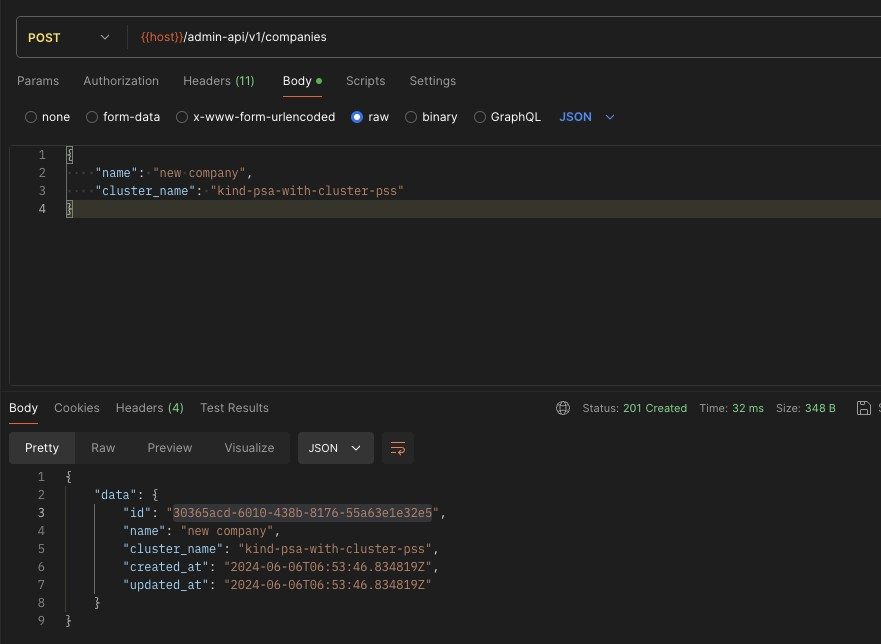
\includegraphics[width=0.8\textwidth]{resources/chapter-4/pengujian/p04-1.jpg}
  \caption{Pembuatan \textit{company} Untuk Pengujian P04}
  \label{fig:pengujian-p04-1}
\end{figure}

\begin{figure}[ht]
  \centering
  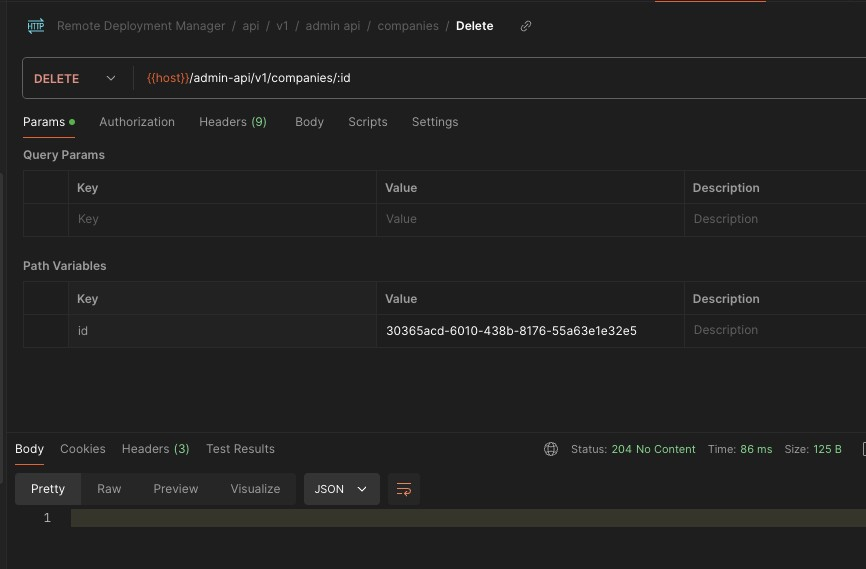
\includegraphics[width=0.8\textwidth]{resources/chapter-4/pengujian/p04.jpg}
  \caption{\textit{Request dan Response Pengujian} P04}
  \label{fig:pengujian-p04}
\end{figure}

\begin{figure}[ht]
  \centering
  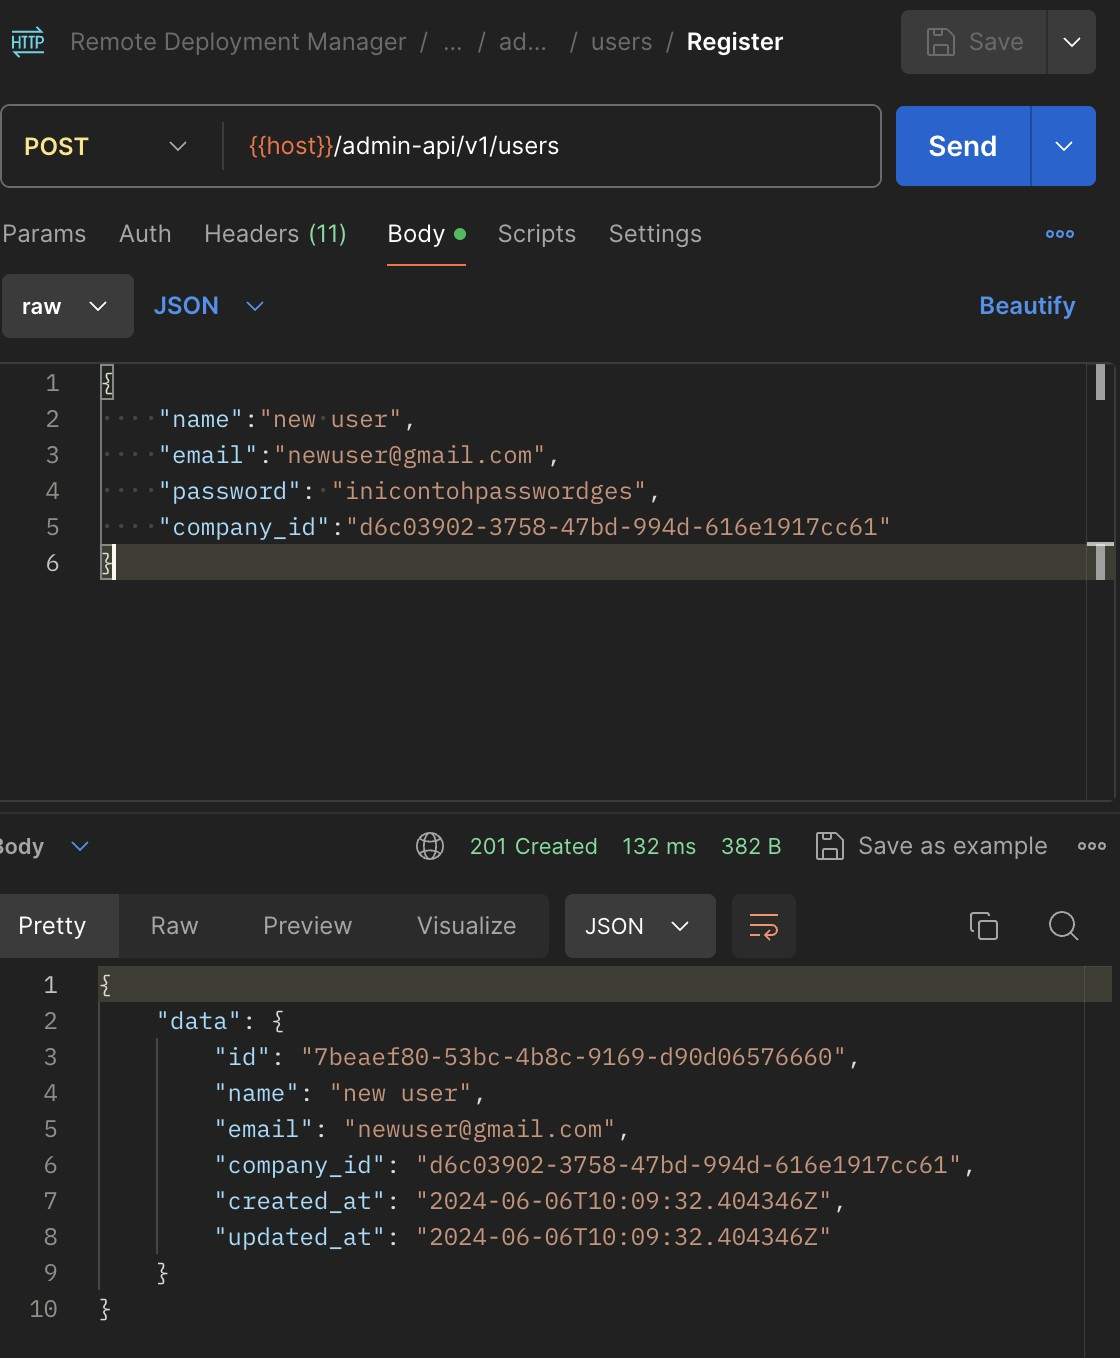
\includegraphics[width=0.8\textwidth]{resources/chapter-4/pengujian/p05.jpg}
  \caption{\textit{Request dan Response Pengujian} P05}
  \label{fig:pengujian-p05}
\end{figure}

\begin{figure}[ht]
  \centering
  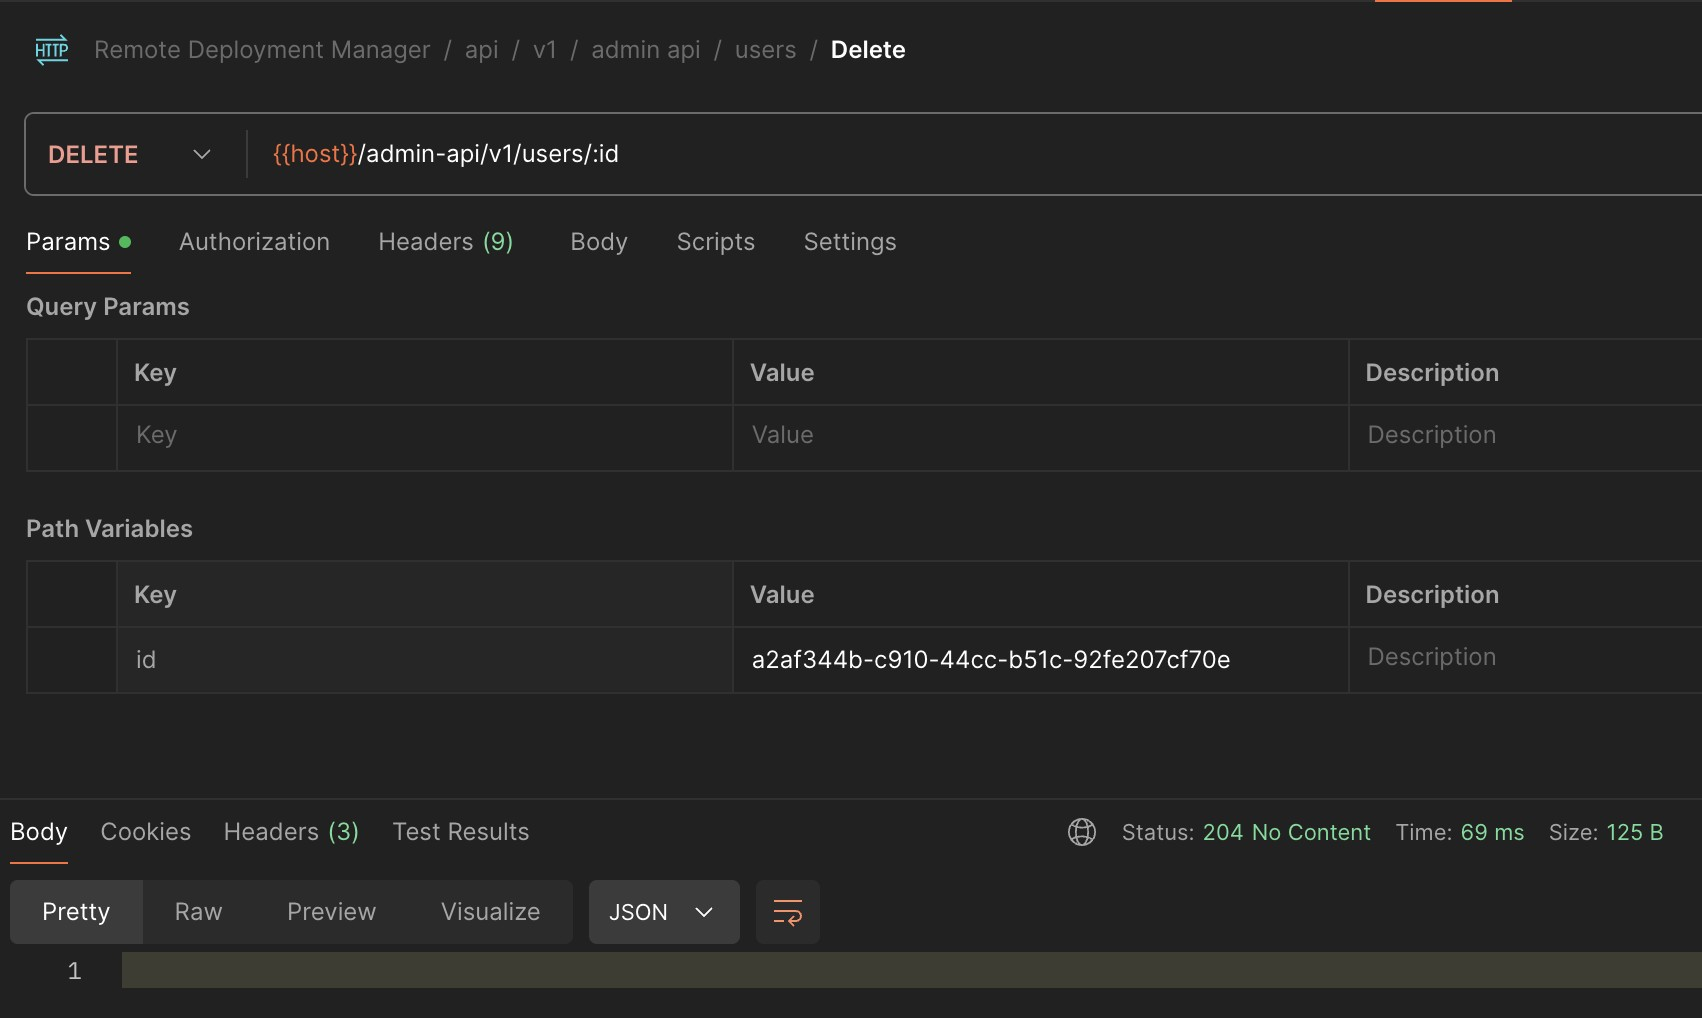
\includegraphics[width=0.8\textwidth]{resources/chapter-4/pengujian/p06.jpg}
  \caption{\textit{Request dan Response Pengujian} P06}
  \label{fig:pengujian-p06}
\end{figure}

\begin{figure}[ht]
  \centering
  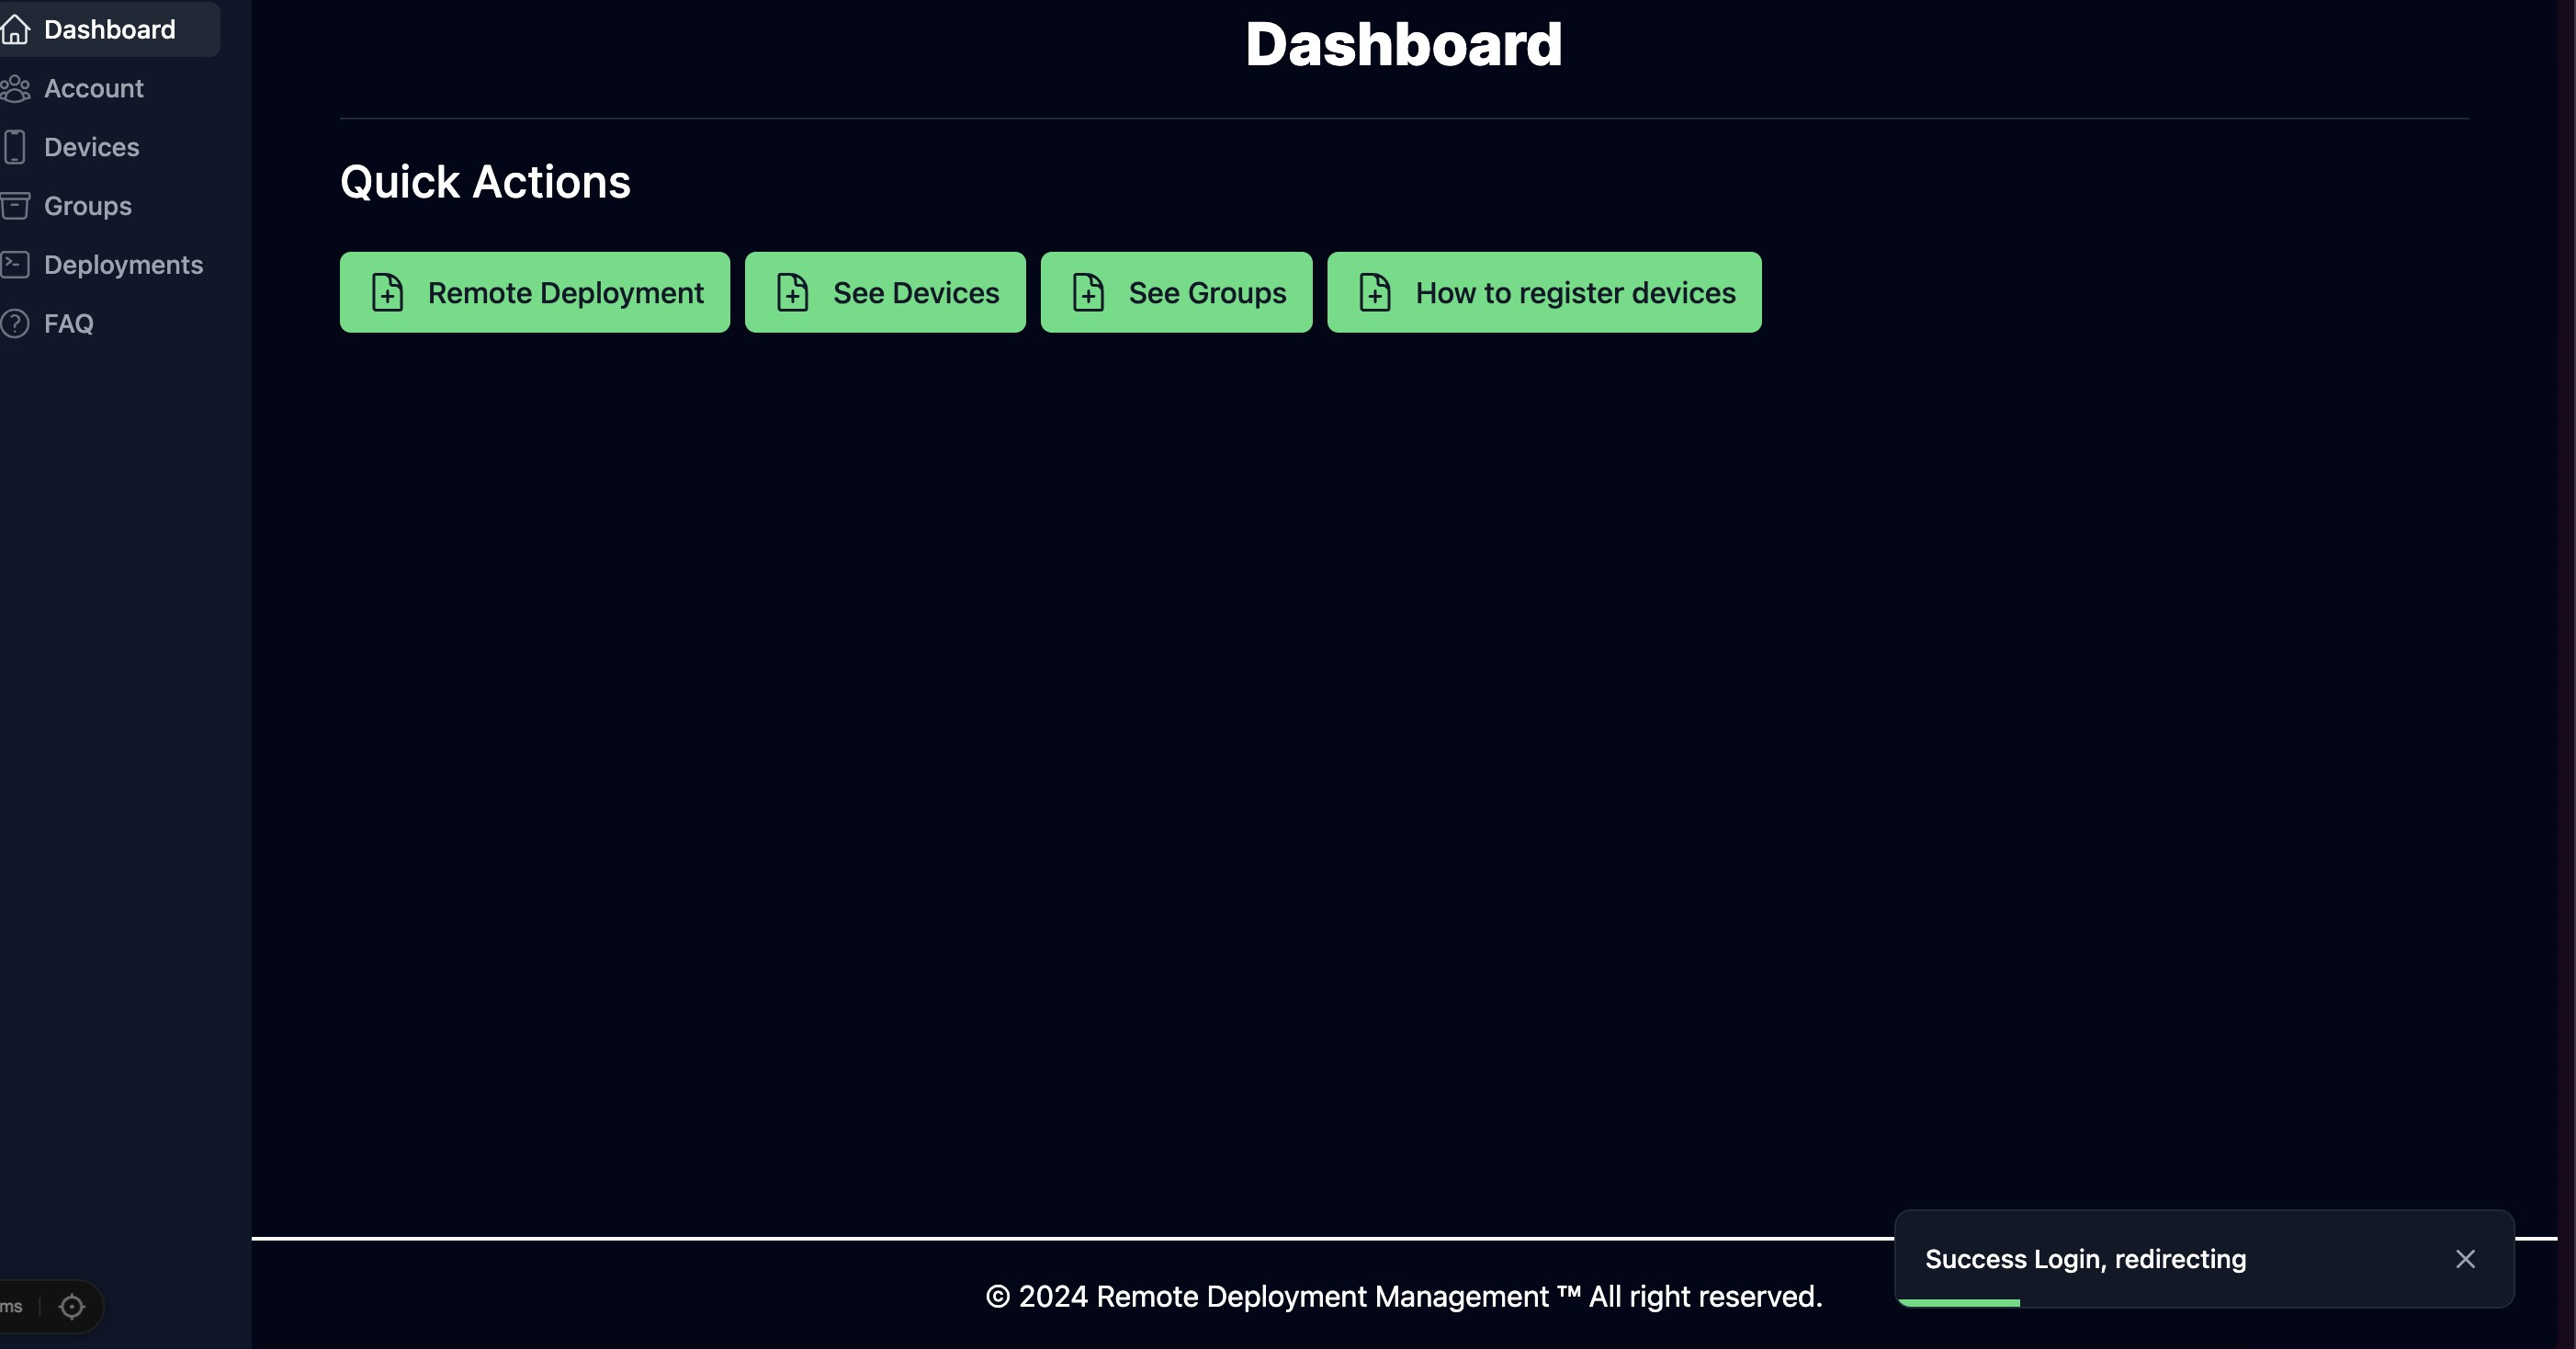
\includegraphics[width=0.8\textwidth]{resources/chapter-4/pengujian/p07.jpg}
  \caption{Redirect ke \textit{Halaman Index} pada Pengujian P07}
  \label{fig:pengujian-p07}
\end{figure}

\begin{figure}[ht]
  \centering
  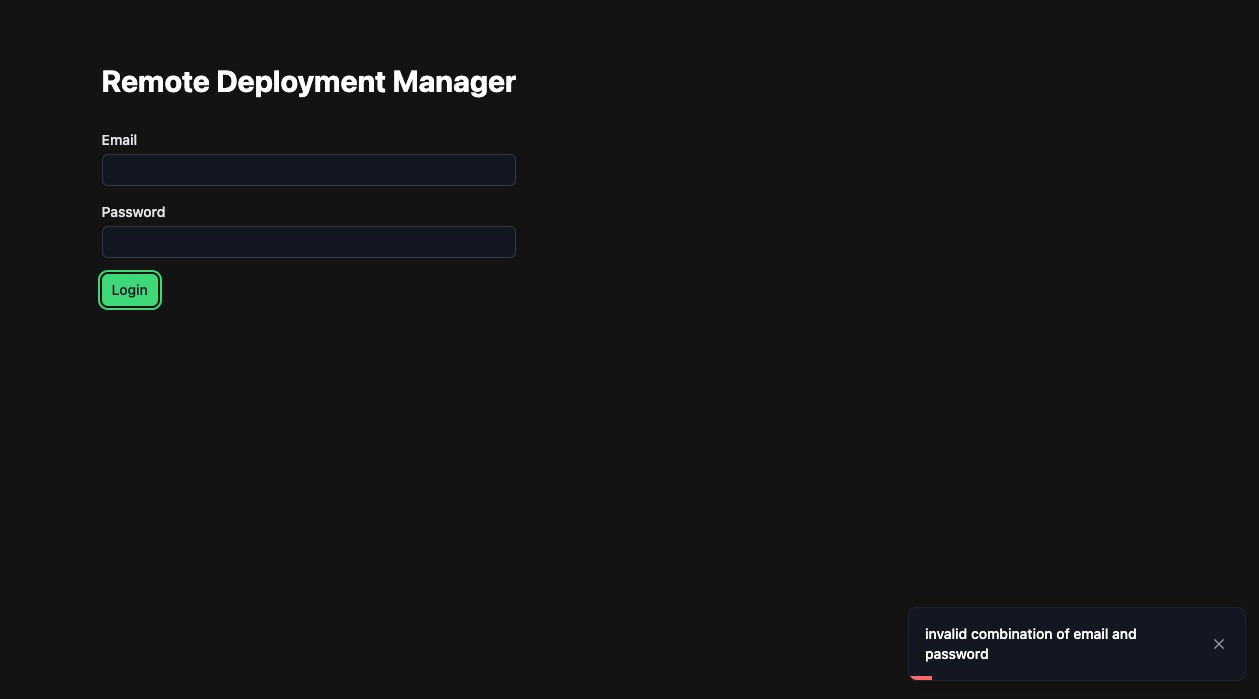
\includegraphics[width=0.8\textwidth]{resources/chapter-4/pengujian/p08.jpg}
  \caption{Muncul Modal Penanda Login Gagal}
  \label{fig:pengujian-p08}
\end{figure}


\begin{figure}[ht]
  \centering
  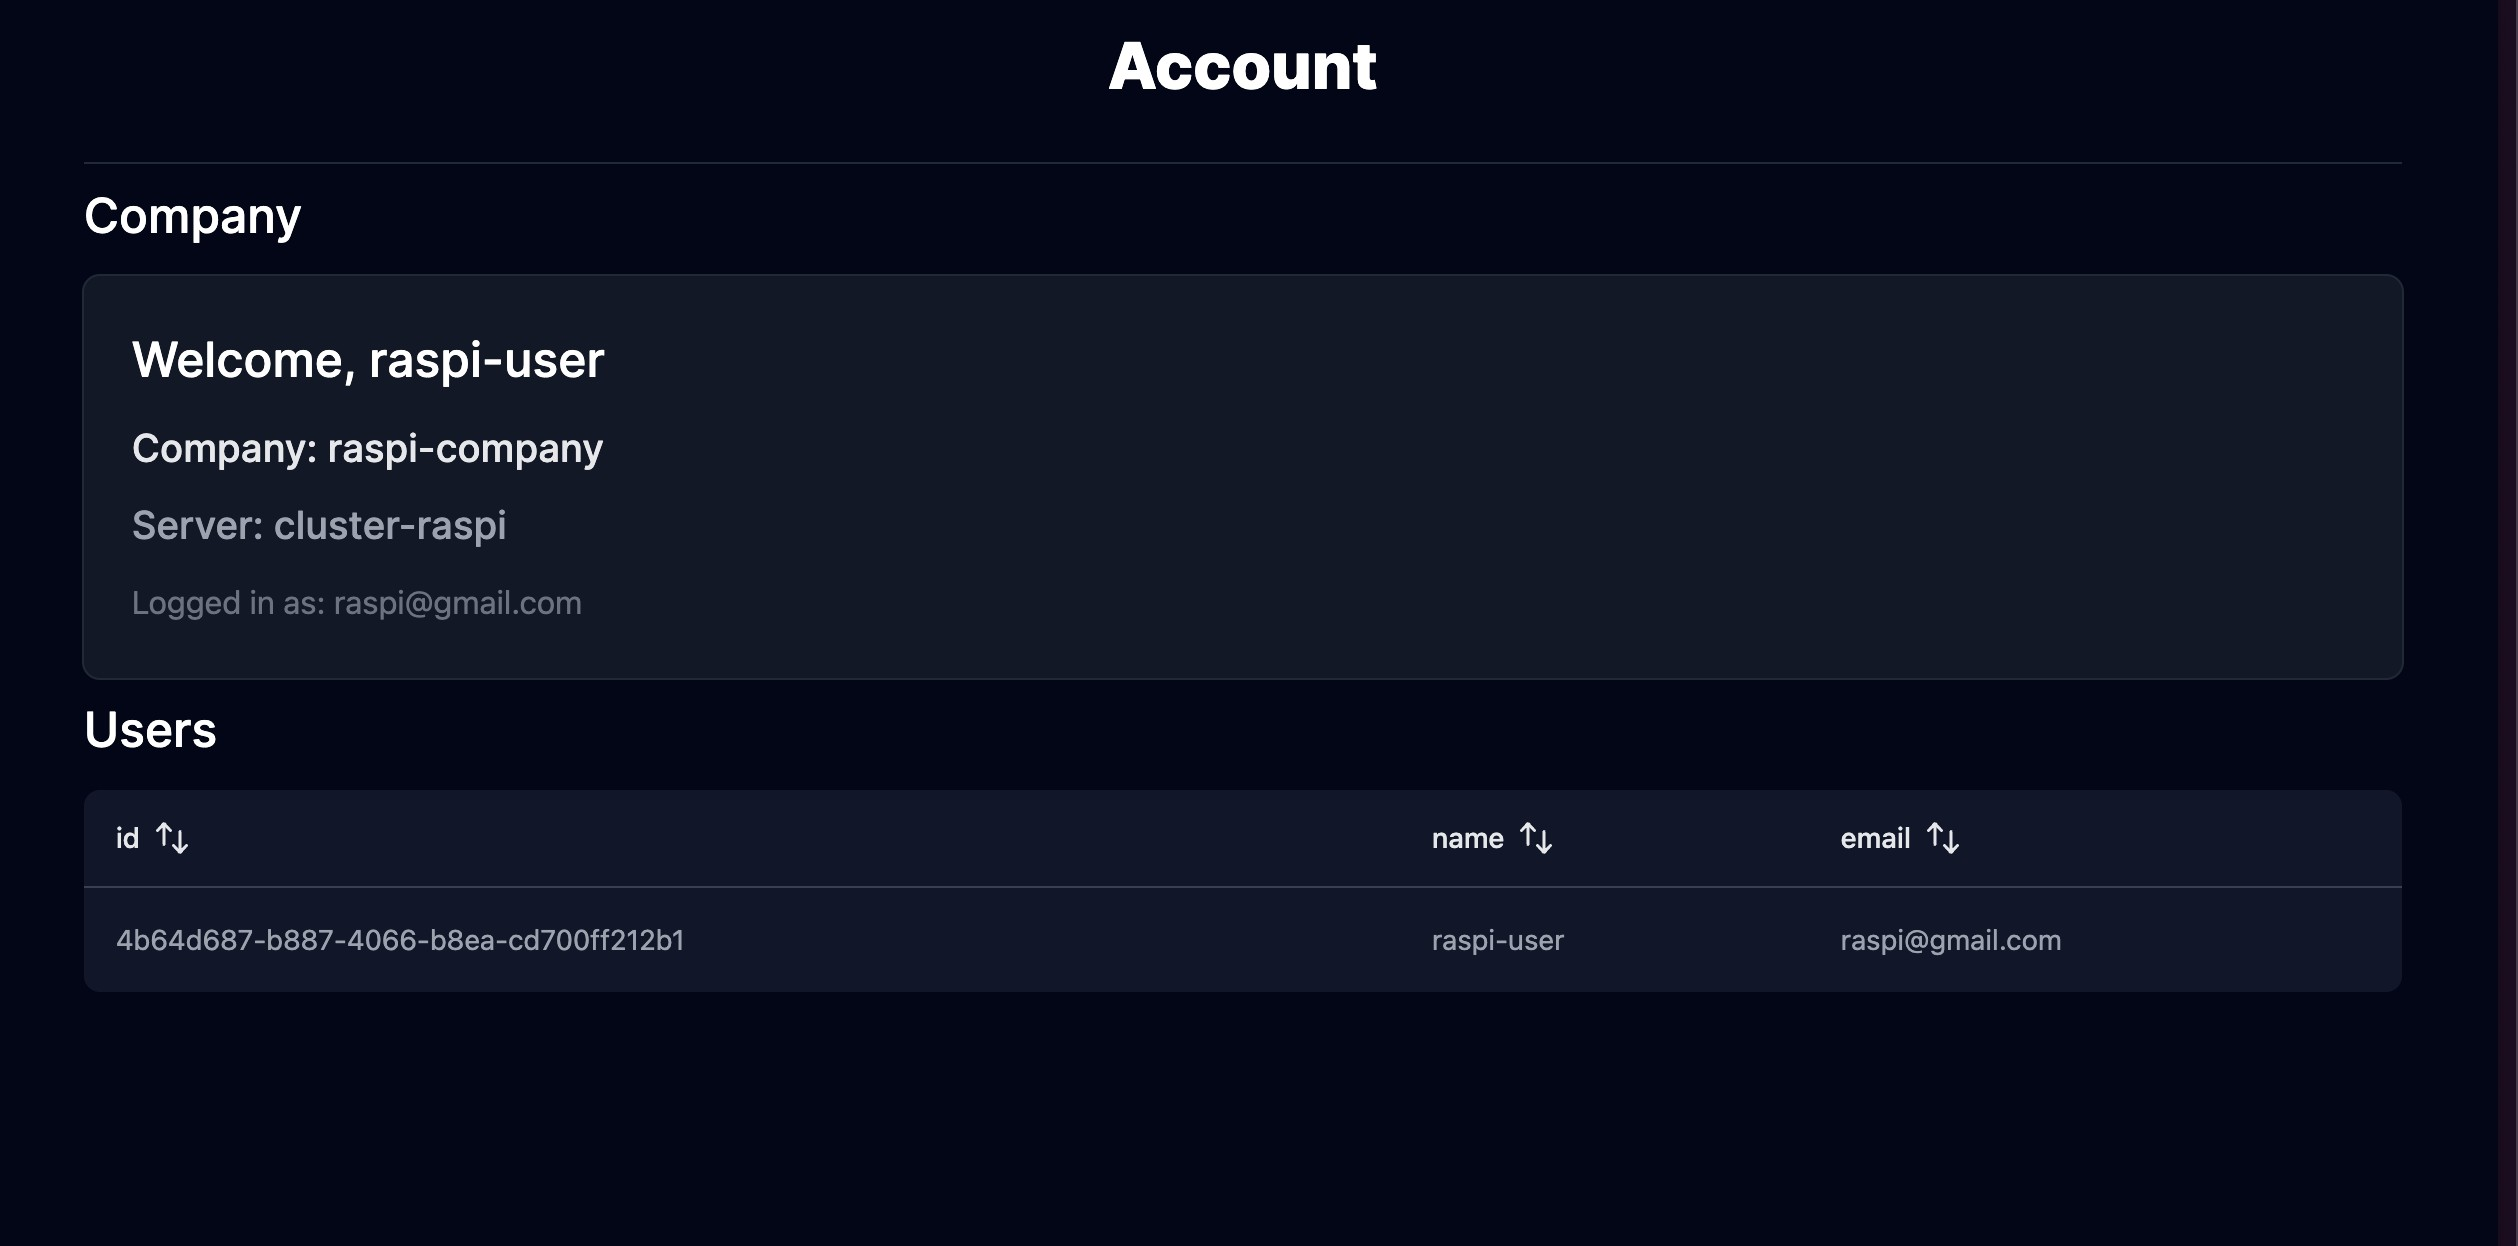
\includegraphics[width=0.8\textwidth]{resources/chapter-4/pengujian/p08-09.jpg}
  \caption{Mengunjungi Halaman Account pada Pengujian P08 dan P09}
  \label{fig:pengujian-p08-09}
\end{figure}

\begin{figure}[ht]
  \centering
  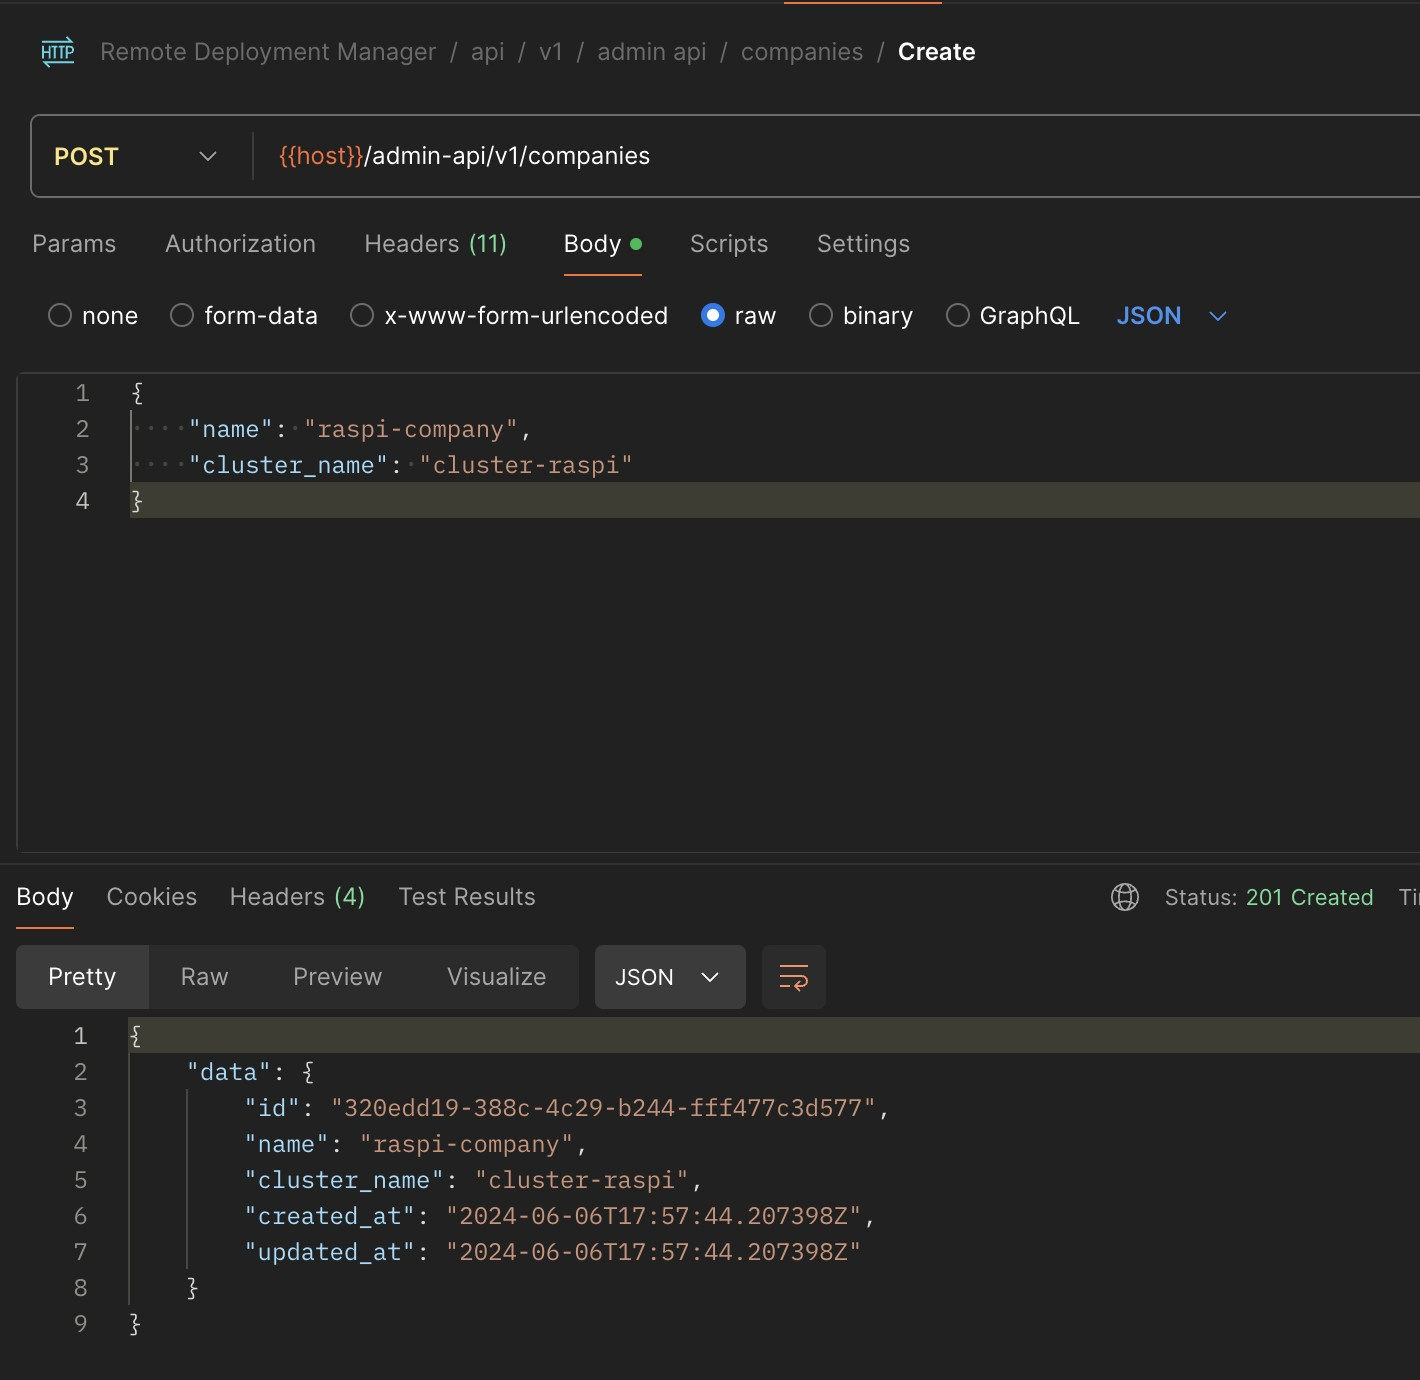
\includegraphics[width=0.8\textwidth]{resources/chapter-4/pengujian/pengujian-sistem-raspi-01.jpg}
  \caption{Pembuatan \textit{Company} Raspi Company}
  \label{fig:pengujian-sistem-raspi-01}
\end{figure}

\begin{figure}[ht]
  \centering
  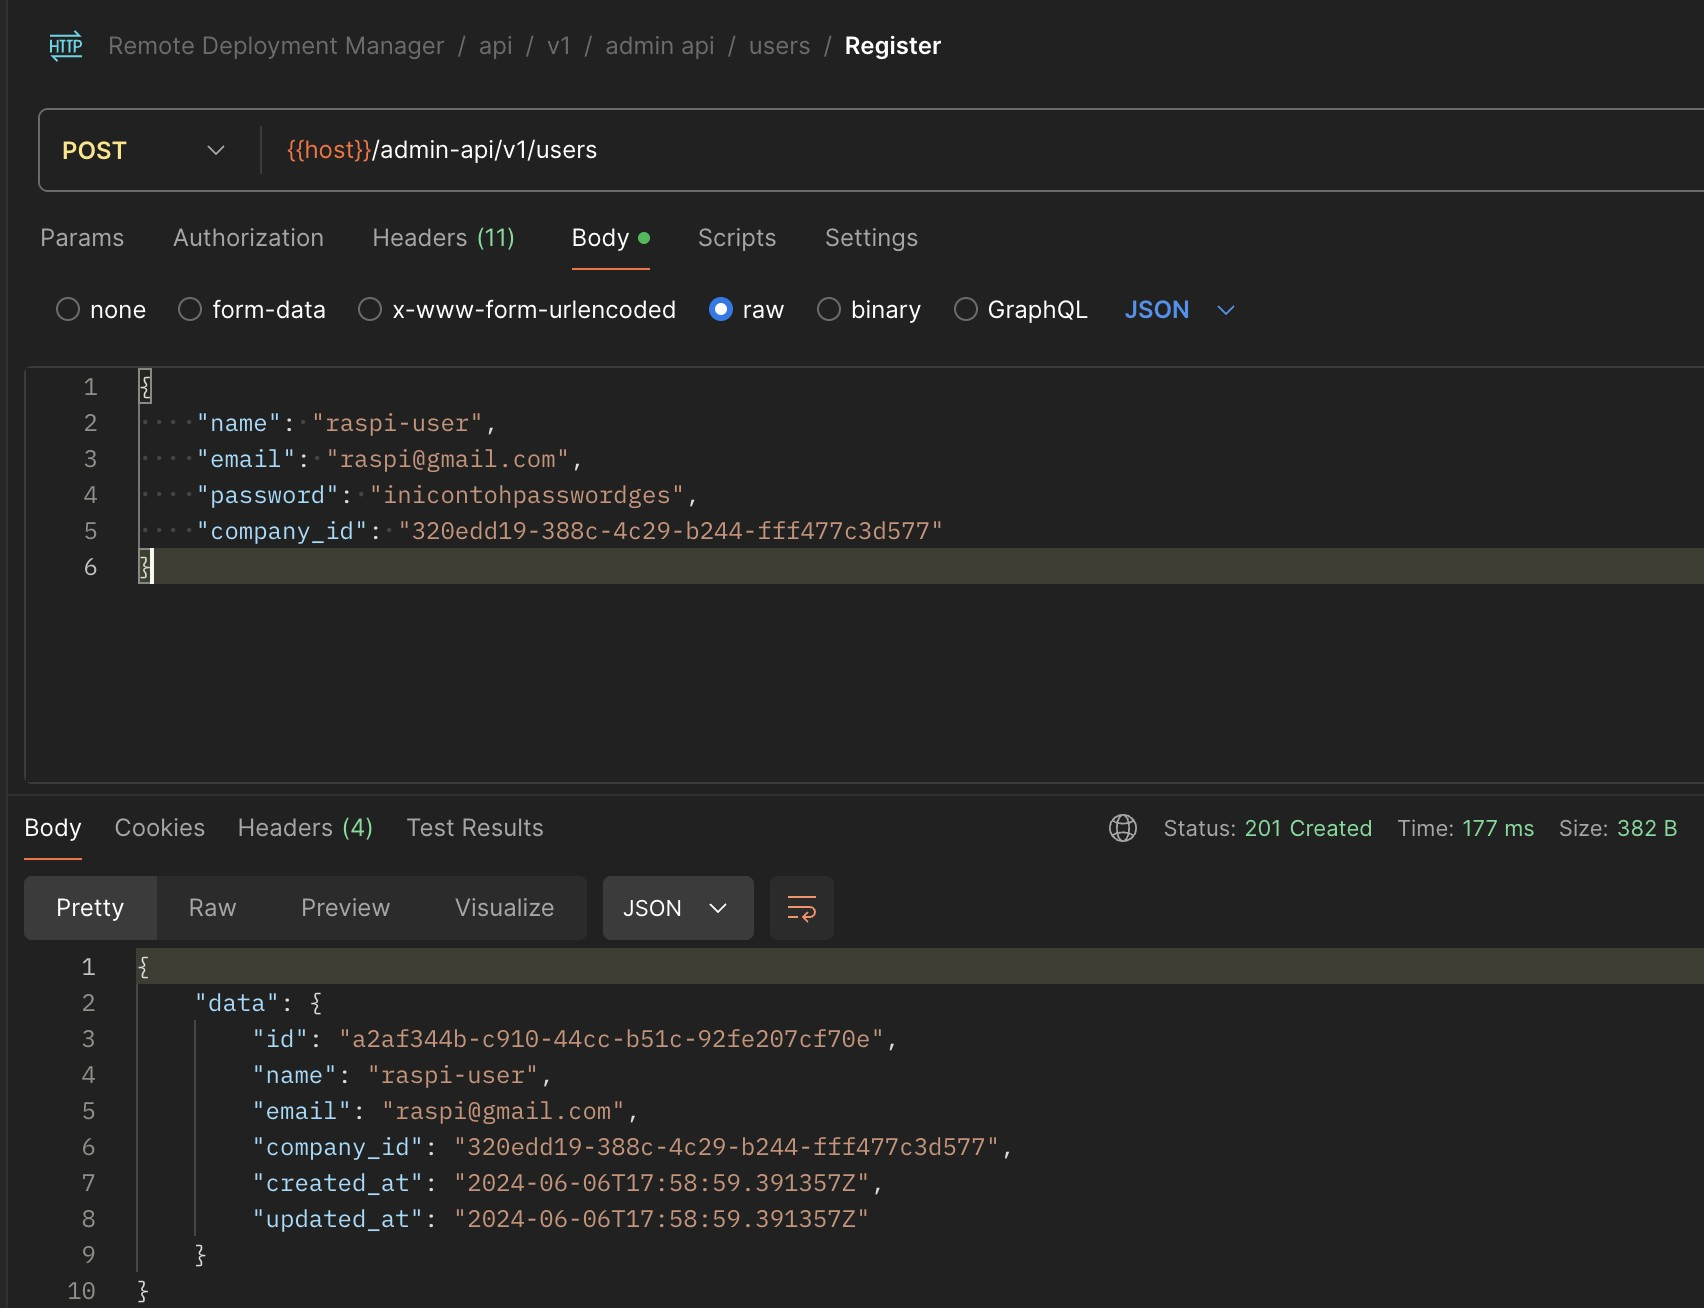
\includegraphics[width=0.8\textwidth]{resources/chapter-4/pengujian/pengujian-sistem-raspi-02.jpg}
  \caption{Pembuatan \textit{User} Raspi-User}
  \label{fig:pengujian-sistem-raspi-02}
\end{figure}

\begin{figure}[ht]
  \centering
  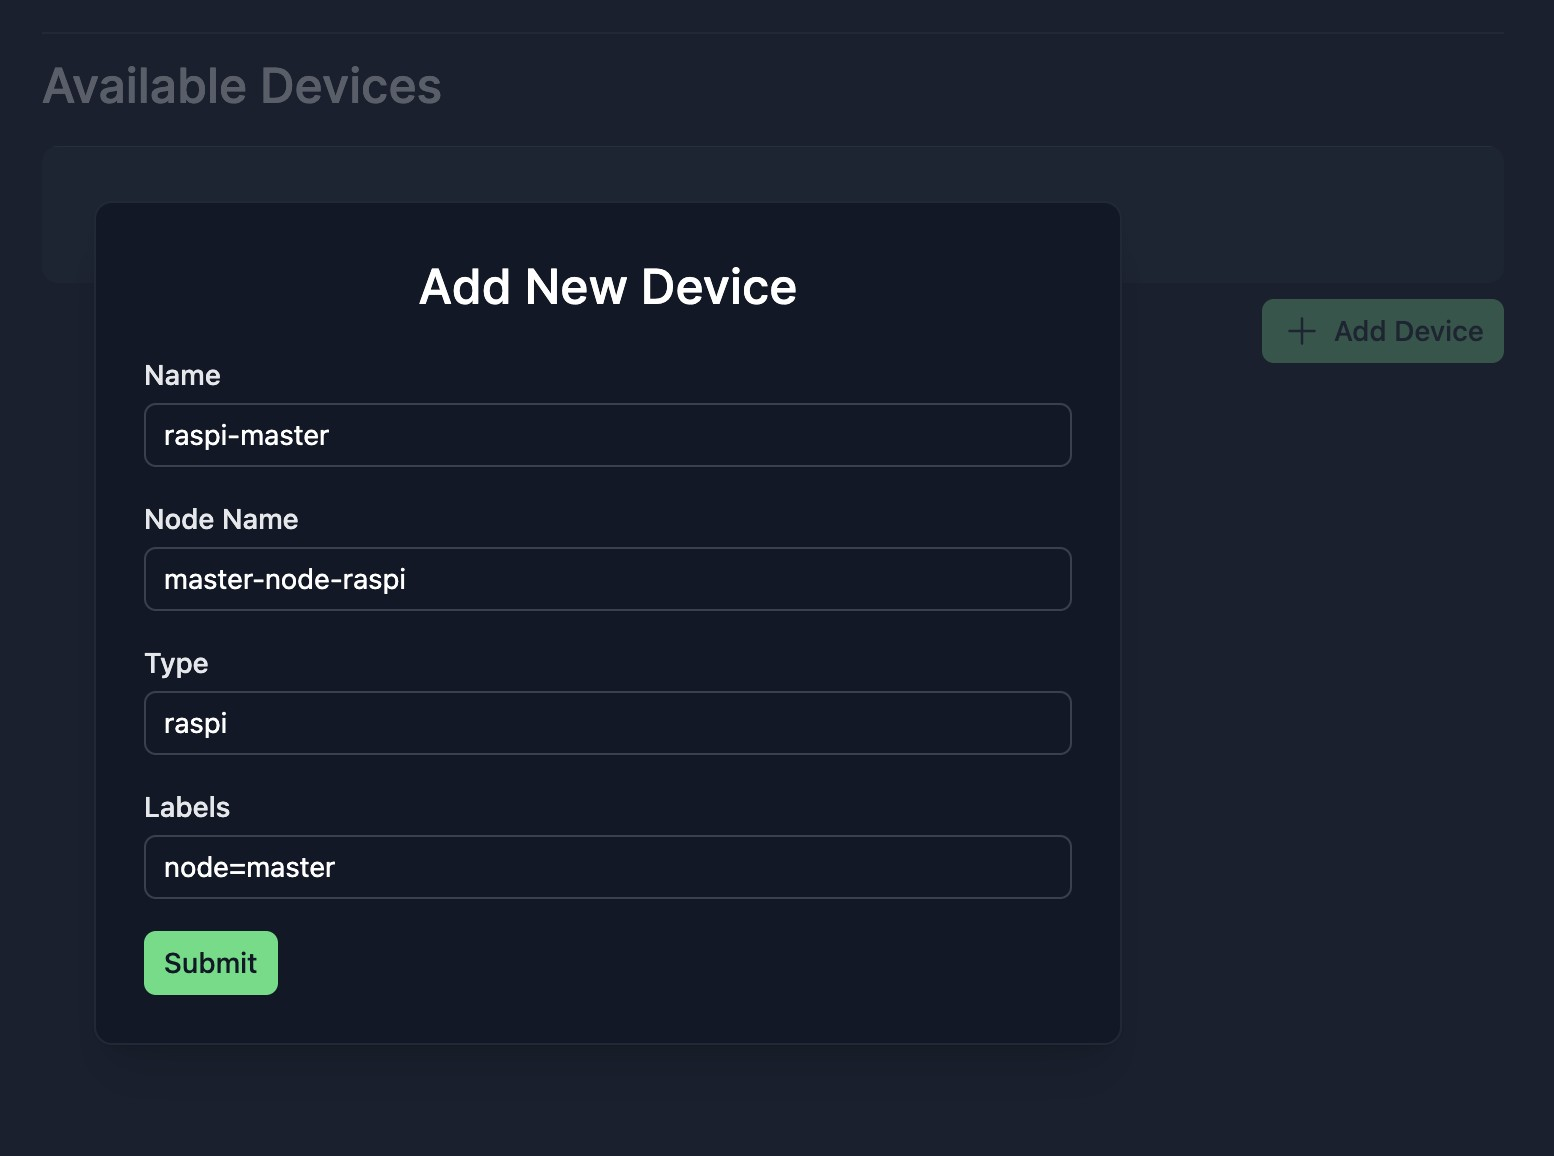
\includegraphics[width=0.8\textwidth]{resources/chapter-4/pengujian/pengujian-sistem-raspi-04-1.jpg}
  \caption{Pembuatan \textit{Device} Raspi}
  \label{fig:pengujian-sistem-raspi-04}
\end{figure}

\begin{figure}[ht]
  \centering
  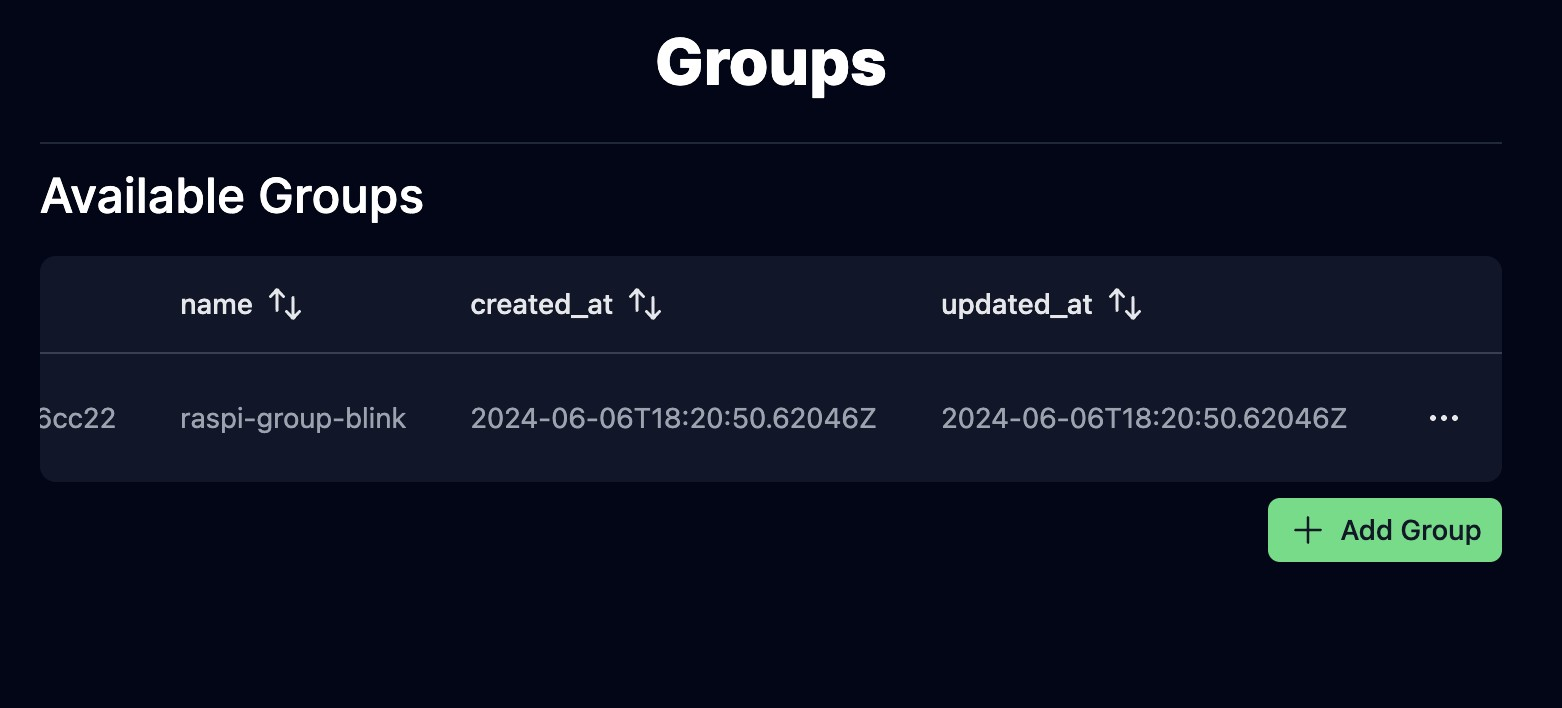
\includegraphics[width=0.8\textwidth]{resources/chapter-4/pengujian/pengujian-sistem-raspi-05.jpg}
  \caption{Pembuatan \textit{Groups} Raspi}
  \label{fig:pengujian-sistem-raspi-05}
\end{figure}

\begin{figure}[ht]
  \centering
  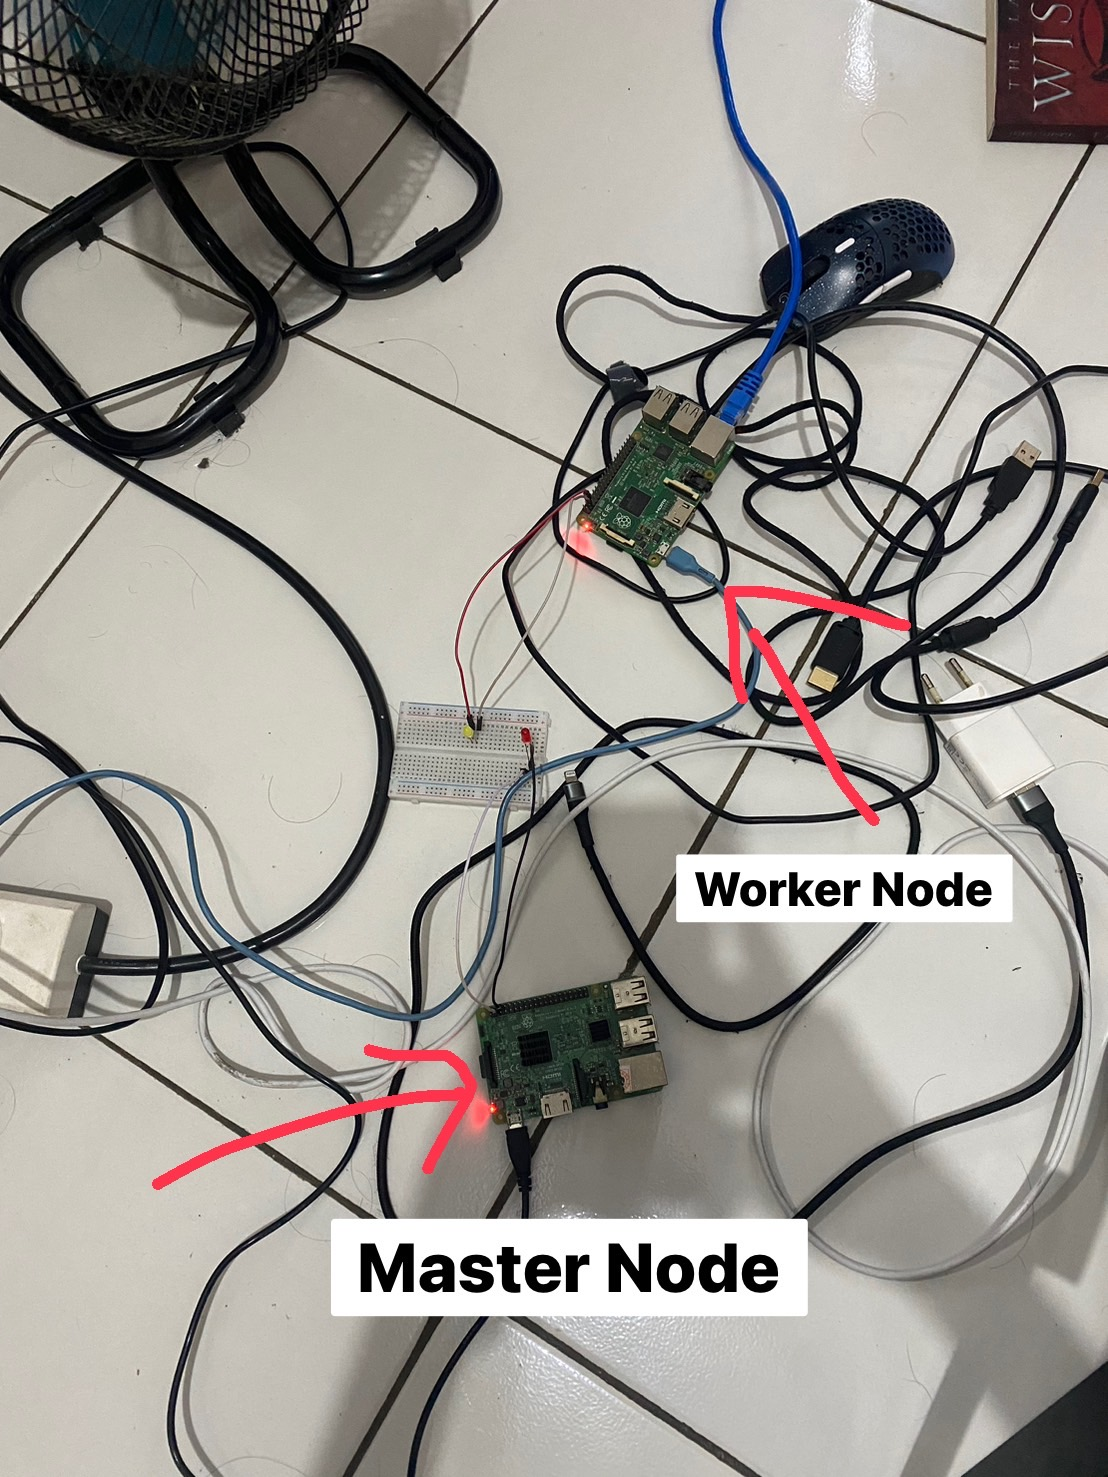
\includegraphics[width=0.8\textwidth]{resources/chapter-4/pengujian/pengujian-sistem-raspi-layout.jpg}
  \caption{Layout Sederhana \textit{Clustser} RaspberryPi}
  \label{fig:pengujian-sistem-raspi-layout}
\end{figure}

\begin{figure}[ht]
  \centering
  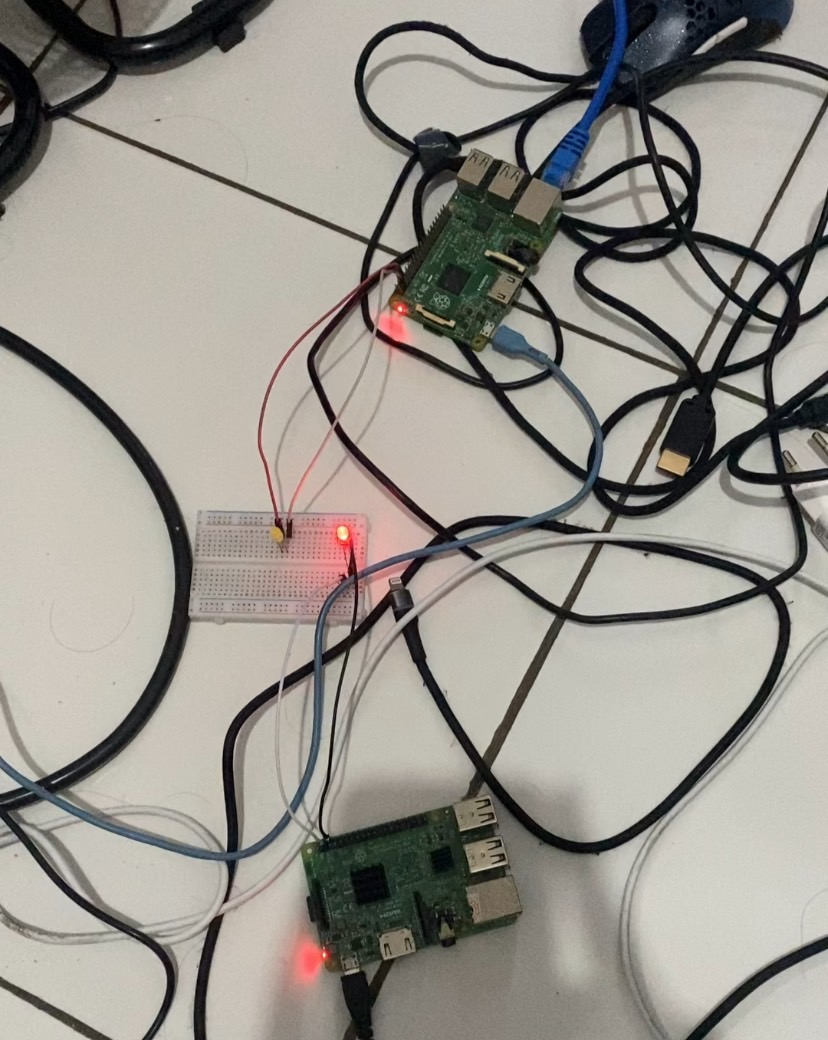
\includegraphics[width=0.8\textwidth]{resources/chapter-4/pengujian/pengujian-sistem-raspi-hasil-a.jpg}
  \caption{Hasil Pengujian Sistem Target Deployment Raspi}
  \label{fig:hasil-pengujian-sistem-raspi-target}
\end{figure}

\begin{figure}[ht]
  \centering
  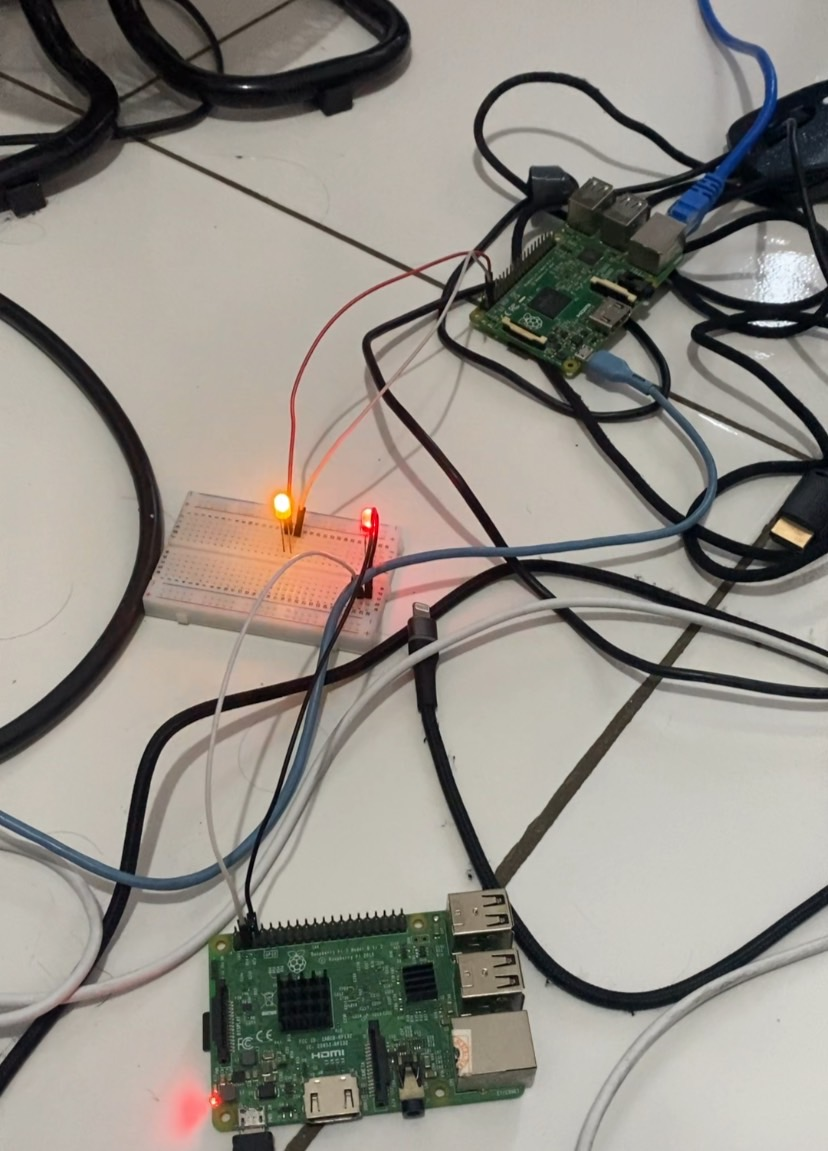
\includegraphics[width=0.8\textwidth]{resources/chapter-4/pengujian/pengujian-sistem-raspi-hasil-b.jpg}
  \caption{Hasil Pengujian Sistem Custom Deployment Raspi}
  \label{fig:hasil-pengujian-sistem-raspi-custom}
\end{figure}

\begin{figure}[ht]
  \centering
  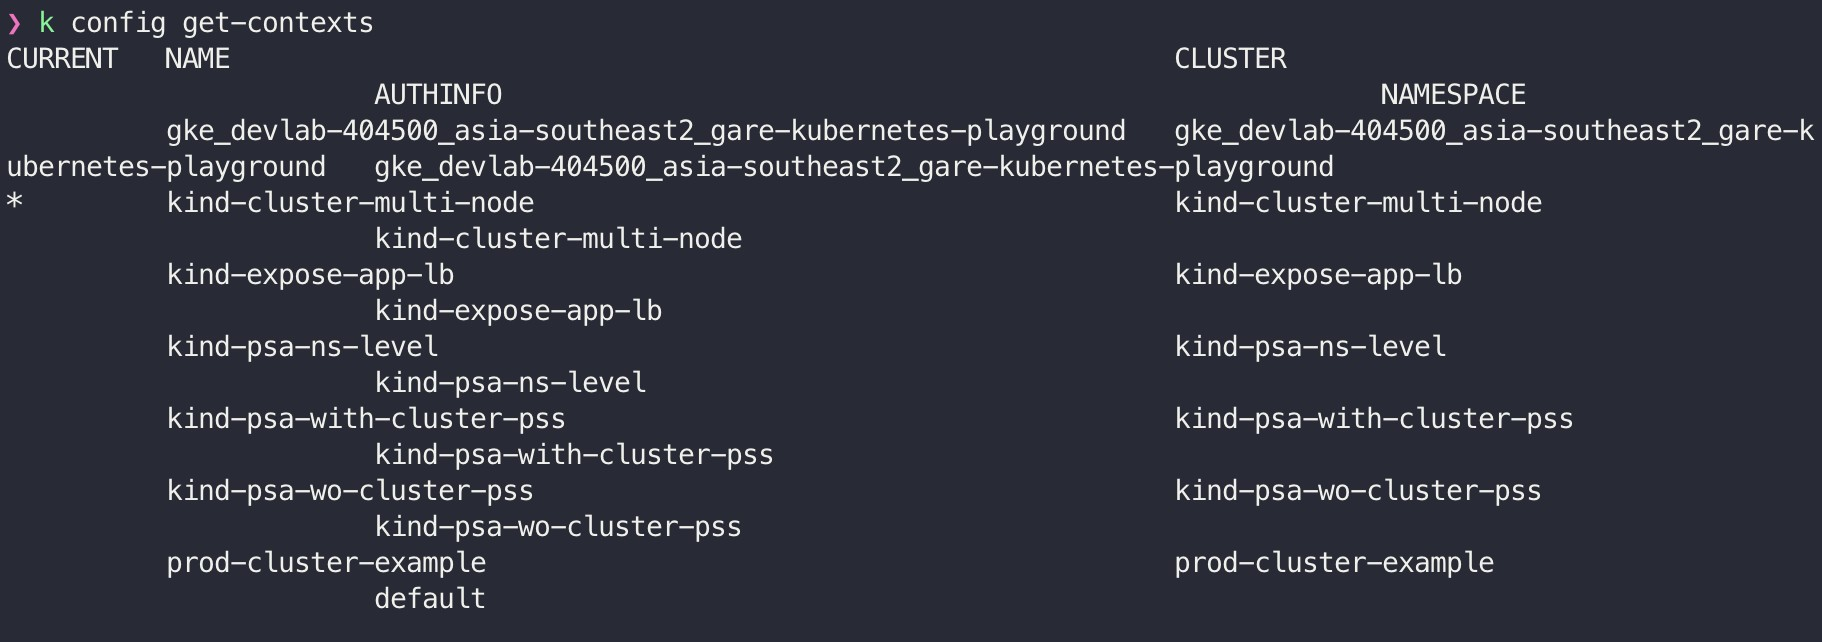
\includegraphics[width=0.8\textwidth]{resources/chapter-4/pengujian/p00.jpg}
  \caption{Daftar Nama Cluster yang Tersedia pada Service}
  \label{fig:list-cluster-tersedia}
\end{figure}


